% -----------------------------------------------------------------------------
% bob: an FPGA built inside an FPGA -- technical deck at the M26 state
%
% RTL structure, configuration, software structure, the flow stage by stage,
% why each choice was made, and bob against OpenFPGA (physical design aside).
%
% Self-contained: every figure is TikZ, no image files. Compiles with pdfLaTeX
% (Overleaf: New Project > Upload Project > this file; compiler pdfLaTeX).
% Fill in \author and \institute below.
%
% Every number comes from the repository at M26 (IDCODE 0x0B026093):
% software/bob/device.json, hw/src/, docs/reports/M26/ (util.rpt, timing.rpt),
% PLAN.md, docs/hwtest/results.log, and the counter and gates examples built at
% M26 (./bob build work/examples/counter/counter.v; ./bob fasm; packets.py).
% -----------------------------------------------------------------------------
\documentclass[aspectratio=169,11pt]{beamer}

\usepackage[T1]{fontenc}
\usepackage{lmodern}
\usepackage{amssymb}
\usepackage{booktabs}
\usepackage{array}
\usepackage{tikz}
\usetikzlibrary{arrows.meta,positioning,calc,fit,backgrounds}

% --- look ---------------------------------------------------------------------
\usetheme{default}
\definecolor{bobteal}{HTML}{0C7A64}     % fabric
\definecolor{bobviolet}{HTML}{6A4DB3}   % configuration
\definecolor{bobamber}{HTML}{E38A1F}    % JTAG, board, highlights
\definecolor{bobblue}{HTML}{2F6DB5}     % software
\definecolor{bobink}{HTML}{16202B}
\definecolor{bobmute}{HTML}{566372}
\definecolor{bobpanel}{HTML}{F2F5F8}
\definecolor{bobclb}{HTML}{DFE7EF}
\definecolor{bobbram}{HTML}{D9ECF7}
\definecolor{bobdsp}{HTML}{F5E4D6}
\definecolor{bobio}{HTML}{E9E4F3}
% chart colours: a validated categorical order (adjacent pairs), light surface
\definecolor{vizA}{HTML}{2A78D6}
\definecolor{vizB}{HTML}{EB6834}
\definecolor{vizC}{HTML}{1BAF7A}
\definecolor{vizD}{HTML}{EDA100}
\definecolor{vizN}{HTML}{C3C6CB}

\setbeamercolor{structure}{fg=bobteal}
\setbeamercolor{normal text}{fg=bobink}
\setbeamercolor{frametitle}{fg=bobink}
\setbeamercolor{alerted text}{fg=bobamber}
\setbeamerfont{frametitle}{series=\bfseries,size=\Large}
\setbeamertemplate{navigation symbols}{}
\setbeamertemplate{itemize items}[circle]
\setbeamertemplate{footline}{%
  \hspace*{1em}{\scriptsize\color{bobmute}\insertsection}\hfill
  {\scriptsize\color{bobmute}bob: an FPGA inside an FPGA \,$\cdot$\, M26\quad\insertframenumber/\inserttotalframenumber}\hspace*{1em}\vspace*{0.6em}}

% a key number and its caption; the caption may hold \\ for a second line
\newcommand{\kpi}[2]{\begin{tabular}[t]{@{}c@{}}{\Large\bfseries\color{bobteal}#1}\\[-2pt]\scriptsize\color{bobmute}\begin{tabular}[t]{@{}c@{}}#2\end{tabular}\end{tabular}}
\newcommand{\src}[1]{{\scriptsize\color{bobmute}#1}}
% a ragged-right paragraph column: no stretched or hyphenated table cells
\newcolumntype{L}[1]{>{\raggedright\arraybackslash}p{#1}}
\newcommand{\mtag}[1]{{\setlength{\fboxsep}{1pt}\colorbox{bobamber!25}{\tiny\bfseries #1}}}
% 0..3 filled dots, for the comparison scorecard
\newcommand{\rate}[1]{\tikz[baseline=-0.6ex]{\foreach \k in {1,2,3}{\ifnum\k>#1\relax\draw[bobmute!70] (\k*0.26,0) circle (0.085);\else\fill[bobteal] (\k*0.26,0) circle (0.085);\fi}}}

\tikzset{
  bx/.style={rounded corners=2pt, align=center, font=\scriptsize, minimum height=7mm, inner sep=2pt},
  blk/.style={bx, draw=bobink!60, fill=bobpanel},
  acc/.style={bx, draw=bobteal, fill=bobteal!12},
  cfg/.style={bx, draw=bobviolet, fill=bobviolet!12},
  hot/.style={bx, draw=bobamber, fill=bobamber!15},
  sw/.style={bx, draw=bobblue, fill=bobblue!10},
  file/.style={bx, draw=bobink!55, dashed, fill=white, font=\tiny\ttfamily, minimum height=6mm},
  mx/.style={draw=bobink!70, fill=white, rounded corners=1.5pt, minimum width=3.5mm, minimum height=7mm, inner sep=1pt, font=\tiny, align=center},
  arr/.style={-{Stealth[length=1.6mm]}, thick, color=bobink!70},
  arr2/.style={{Stealth[length=1.6mm]}-{Stealth[length=1.6mm]}, thick, color=bobink!70},
  bus/.style={-{Stealth[length=1.6mm]}, line width=1.2pt, color=bobink!60},
  tree/.style={draw=bobink!45, thick},
  lbl/.style={font=\tiny, color=bobmute},
  sm/.style={minimum height=4.3mm, inner sep=1.5pt, font=\tiny},
}

\title{bob: an FPGA built inside an FPGA}
\subtitle{RTL and software structure, the flow stage by stage,\\and how it compares with OpenFPGA\\[3pt]
  {\small state of milestone M26 \,$\cdot$\, IDCODE \texttt{0x0B026093} \,$\cdot$\, 74/74 on the board}}
\author{Your Name}            % <- fill in
\institute{Your Institute}    % <- fill in
\date{September 2026}

\begin{document}

% =============================================================================
\begin{frame}[plain]
  \titlepage
\end{frame}

% =============================================================================
\begin{frame}{Roadmap}
  \centering
  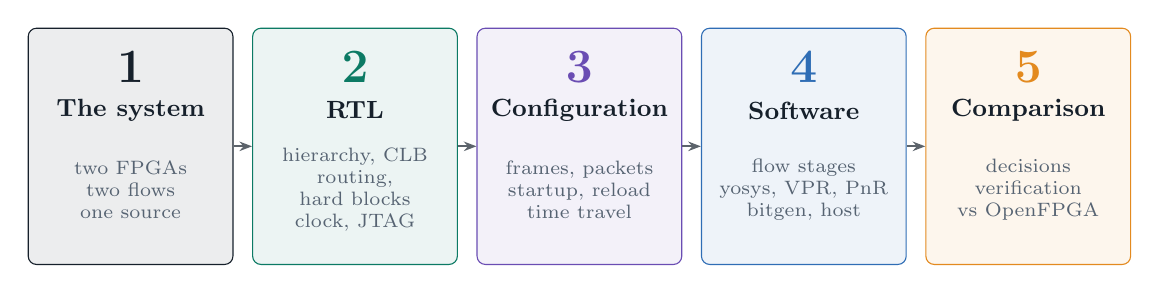
\begin{tikzpicture}[font=\scriptsize]
    \foreach \n/\x/\ti/\su/\col in {
      1/0/{The system}/{two FPGAs\\two flows\\one source}/bobink,
      2/2.85/{RTL}/{hierarchy, CLB\\routing, hard blocks\\clock, JTAG}/bobteal,
      3/5.7/{Configuration}/{frames, packets\\startup, reload\\time travel}/bobviolet,
      4/8.55/{Software}/{flow stages\\yosys, VPR, PnR\\bitgen, host}/bobblue,
      5/11.4/{Comparison}/{decisions\\verification\\vs OpenFPGA}/bobamber}
    {
      \node[draw=\col, fill=\col!8, rounded corners=3pt, minimum width=26mm, minimum height=30mm] (b\n) at (\x,0) {};
      \node[font=\LARGE\bfseries, text=\col] at ($(b\n.north)+(0,-0.5)$) {\n};
      \node[font=\small\bfseries, text=bobink] at ($(b\n.north)+(0,-1.05)$) {\ti};
      \node[font=\scriptsize, text=bobmute, align=center, text width=23mm] at ($(b\n.center)+(0,-0.55)$) {\su};
    }
    \foreach \a/\b in {1/2,2/3,3/4,4/5} \draw[arr] (b\a.east) -- (b\b.west);
  \end{tikzpicture}
  \vspace{6mm}

  \small Running example on every slide: \texttt{work/examples/counter/counter.v}, a 6-bit counter with enable and synchronous reset, built at M26.
\end{frame}

% =============================================================================
\section{The system}
\begin{frame}{The system: two FPGAs, two flows}
  \centering
  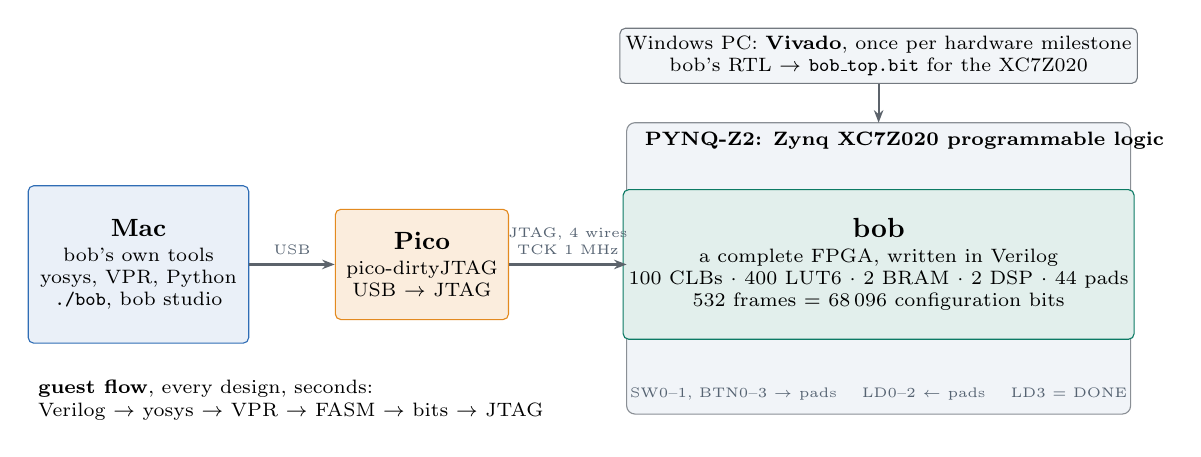
\begin{tikzpicture}[font=\scriptsize]
    \node[sw, minimum width=28mm, minimum height=20mm] (mac) at (1.4,2.4) {\small\textbf{Mac}\\[1pt]bob's own tools\\yosys, VPR, Python\\\texttt{./bob}, bob studio};
    \node[hot, minimum width=22mm, minimum height=14mm] (pico) at (5.0,2.4) {\small\textbf{Pico}\\[1pt]pico-dirtyJTAG\\USB $\rightarrow$ JTAG};
    \draw[fill=bobclb!45, draw=bobink!50, rounded corners=3pt] (7.6,0.5) rectangle (14,4.2);
    \node[anchor=north west, font=\scriptsize\bfseries] at (7.6,4.2) {\ PYNQ-Z2: Zynq XC7Z020 programmable logic};
    \node[acc, minimum width=54mm, minimum height=19mm] (bob) at (10.8,2.4) {\normalsize\textbf{bob}\\[1pt]a complete FPGA, written in Verilog\\100 CLBs $\cdot$ 400 LUT6 $\cdot$ 2 BRAM $\cdot$ 2 DSP $\cdot$ 44 pads\\532 frames = 68\,096 configuration bits};
    \node[lbl, anchor=south] at (10.8,0.55) {SW0--1, BTN0--3 $\rightarrow$ pads \quad LD0--2 $\leftarrow$ pads \quad LD3 = DONE};
    \node[blk, minimum width=58mm] (viv) at (10.8,5.05) {Windows PC: \textbf{Vivado}, once per hardware milestone\\bob's RTL $\rightarrow$ \texttt{bob\_top.bit} for the XC7Z020};
    \draw[arr] (mac) -- node[above, lbl]{USB} (pico);
    \draw[arr] (pico) -- node[above, lbl, align=center]{JTAG, 4 wires\\TCK 1 MHz} (7.6,2.4);
    \draw[arr] (viv) -- (10.8,4.2);
    \node[font=\scriptsize, align=left, anchor=north west] at (0,1.05) {\textbf{guest flow}, every design, seconds:\\Verilog $\rightarrow$ yosys $\rightarrow$ VPR $\rightarrow$ FASM $\rightarrow$ bits $\rightarrow$ JTAG};
  \end{tikzpicture}
  \vspace{3mm}

  \kpi{400}{LUT6 in 100 CLBs}\hfill
  \kpi{68\,096}{configuration bits}\hfill
  \kpi{8\,095}{configurable muxes}\hfill
  \kpi{3.4\,s}{\texttt{counter.v} $\rightarrow$ \texttt{.bit}}\hfill
  \kpi{74/74}{board checks at M26}
\end{frame}

% =============================================================================
\begin{frame}{The repository: who makes what}
  \centering
  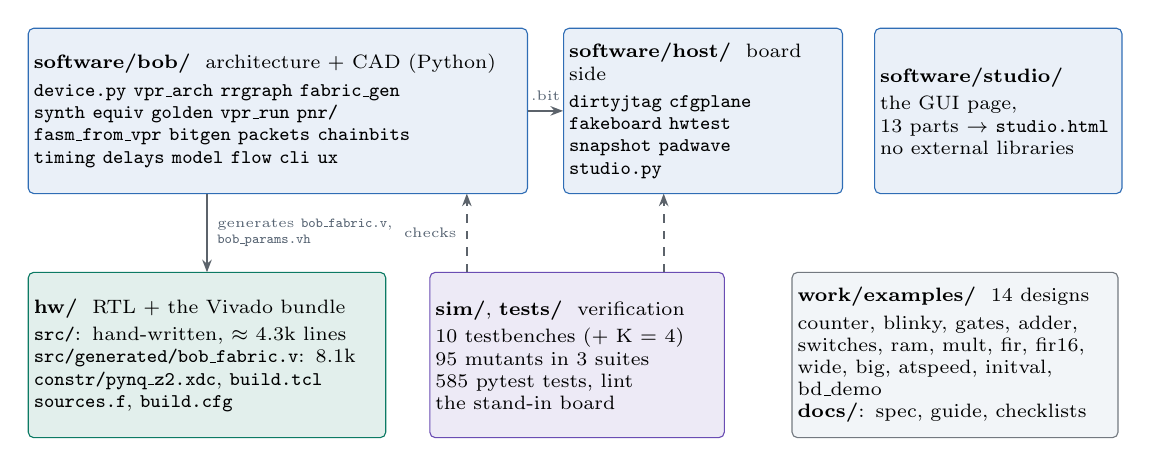
\begin{tikzpicture}[font=\scriptsize]
    \node[sw, text width=62mm, align=left, minimum height=21mm] (sb) at (3.2,4.3) {\textbf{software/bob/}\ \ architecture + CAD (Python)\\[2pt]
      \texttt{device.py vpr\_arch rrgraph fabric\_gen}\\
      \texttt{synth equiv golden vpr\_run pnr/}\\
      \texttt{fasm\_from\_vpr bitgen packets chainbits}\\
      \texttt{timing delays model flow cli ux}};
    \node[sw, text width=34mm, align=left, minimum height=21mm] (sh) at (8.6,4.3) {\textbf{software/host/}\ \ board side\\[2pt]
      \texttt{dirtyjtag cfgplane}\\\texttt{fakeboard hwtest}\\\texttt{snapshot padwave}\\\texttt{studio.py}};
    \node[sw, text width=30mm, align=left, minimum height=21mm] (ss) at (12.35,4.3) {\textbf{software/studio/}\\[2pt]the GUI page,\\13 parts $\rightarrow$ \texttt{studio.html}\\no external libraries};
    \node[acc, text width=44mm, align=left, minimum height=21mm] (hw) at (2.3,1.2) {\textbf{hw/}\ \ RTL + the Vivado bundle\\[2pt]
      \texttt{src/}: hand-written, $\approx$ 4.3k lines\\
      \texttt{src/generated/bob\_fabric.v}: 8.1k\\
      \texttt{constr/pynq\_z2.xdc}, \texttt{build.tcl}\\
      \texttt{sources.f}, \texttt{build.cfg}};
    \node[cfg, text width=36mm, align=left, minimum height=21mm] (vt) at (7.0,1.2) {\textbf{sim/}, \textbf{tests/}\ \ verification\\[2pt]
      10 testbenches (+ K = 4)\\95 mutants in 3 suites\\585 pytest tests, lint\\the stand-in board};
    \node[blk, text width=40mm, align=left, minimum height=21mm] (ex) at (11.8,1.2) {\textbf{work/examples/}\ \ 14 designs\\[2pt]
      counter, blinky, gates, adder,\\switches, ram, mult, fir, fir16,\\wide, big, atspeed, initval, bd\_demo\\
      \textbf{docs/}: spec, guide, checklists};
    \draw[arr] (2.3,3.25) -- node[right, lbl, align=left]{generates \texttt{bob\_fabric.v},\\\texttt{bob\_params.vh}} (2.3,2.25);
    \draw[arr] (sb.east) -- node[above, lbl]{.bit} (sb.east -| sh.west);
    \draw[arr, dashed] (5.6,2.25) -- node[left, lbl]{checks} (5.6,3.25);
    \draw[arr, dashed] (8.1,2.25) -- (8.1,3.25);
  \end{tikzpicture}
  \vspace{2mm}

  \src{Python 27k lines $\cdot$ Verilog 7.5k (+ 8.1k generated) $\cdot$ JavaScript 4.6k $\cdot$ Tcl 1.4k $\cdot$ 116 commits, tags \texttt{m7} \dots\ \texttt{m26}}
\end{frame}

% =============================================================================
\begin{frame}{One description generates everything: \texttt{device.py}}
  \centering
  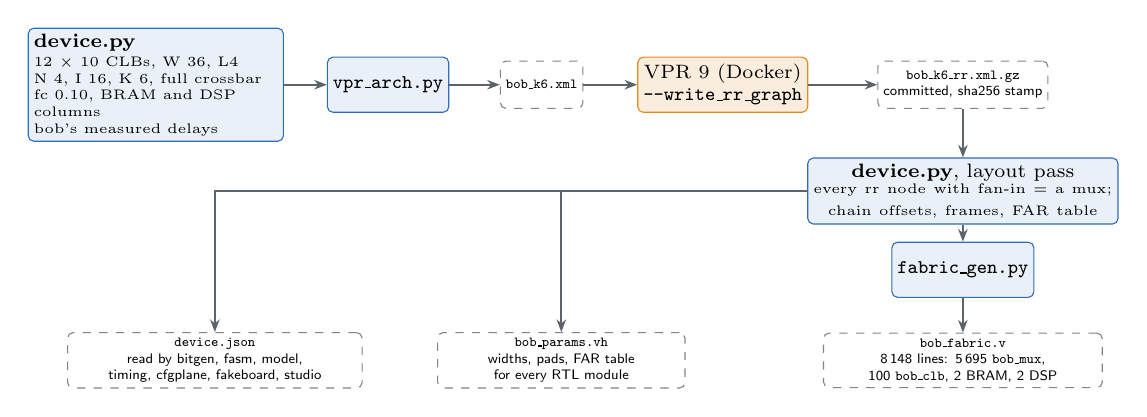
\begin{tikzpicture}[font=\scriptsize]
    \node[sw, text width=31mm, align=left, font=\tiny] (dev) at (1.65,4.1) {{\scriptsize\textbf{device.py}}\\[1pt]12 $\times$ 10 CLBs, W 36, L4\\N 4, I 16, K 6, full crossbar\\fc 0.10, BRAM and DSP columns\\bob's measured delays};
    \node[sw] (va) at (4.6,4.1) {\texttt{vpr\_arch.py}};
    \node[file] (ax) at (6.55,4.1) {bob\_k6.xml};
    \node[hot] (vpr) at (8.85,4.1) {VPR 9 (Docker)\\\texttt{-{}-write\_rr\_graph}};
    \node[file] (rr) at (11.9,4.1) {bob\_k6\_rr.xml.gz\\\sffamily committed, sha256 stamp};
    \node[sw, text width=38mm] (lay) at (11.9,2.75) {\textbf{device.py}, layout pass\\\tiny every rr node with fan-in = a mux;\\\tiny chain offsets, frames, FAR table};
    \node[sw] (fg) at (11.9,1.75) {\texttt{fabric\_gen.py}};
    \node[file, text width=34mm] (fab) at (11.9,0.6) {bob\_fabric.v\\\sffamily 8\,148 lines: 5\,695 \texttt{bob\_mux},\\\sffamily 100 \texttt{bob\_clb}, 2 BRAM, 2 DSP};
    \node[file, text width=36mm] (dj) at (2.4,0.6) {device.json\\\sffamily read by bitgen, fasm, model,\\\sffamily timing, cfgplane, fakeboard, studio};
    \node[file, text width=30mm] (vh) at (6.8,0.6) {bob\_params.vh\\\sffamily widths, pads, FAR table\\\sffamily for every RTL module};
    \draw[arr] (dev) -- (va); \draw[arr] (va) -- (ax); \draw[arr] (ax) -- (vpr); \draw[arr] (vpr) -- (rr);
    \draw[arr] (rr) -- (lay); \draw[arr] (lay) -- (fg); \draw[arr] (fg) -- (fab);
    \draw[arr] (lay.west) -| (vh.north);
    \draw[arr] (lay.west) -| (dj.north);
  \end{tikzpicture}
  \vspace{2mm}

  \small Change the grid: edit one dictionary, then \texttt{make rrgraph} $\rightarrow$ \texttt{make device} $\rightarrow$ \texttt{make vpr}.\\
  The router's graph and the hardware are one object: every route VPR finds exists in the RTL.
\end{frame}

% =============================================================================
\section{RTL}
\begin{frame}{RTL: module hierarchy of the board build}
  \centering
  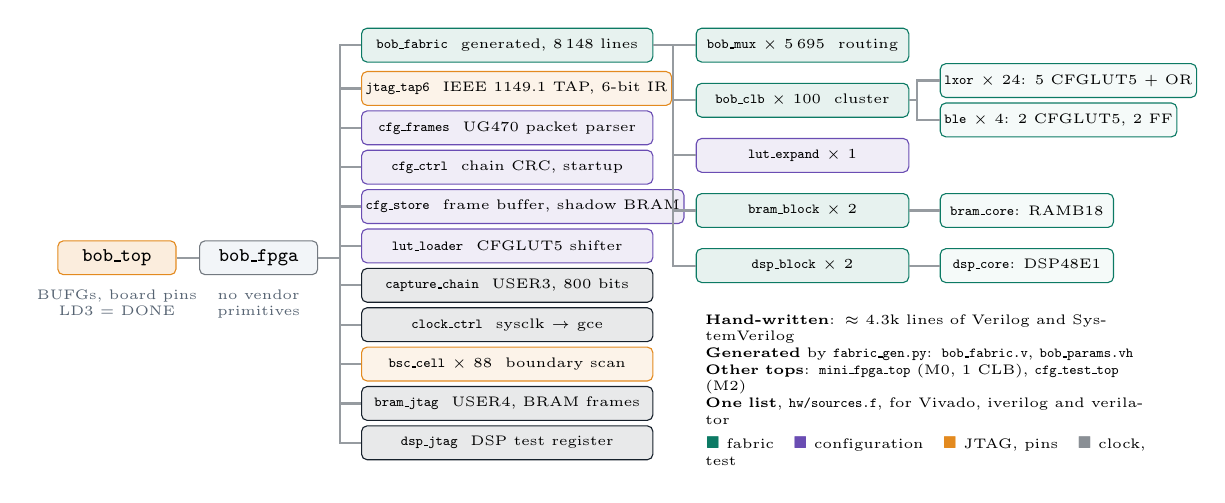
\begin{tikzpicture}[font=\tiny]
    \node[hot, sm, minimum width=15mm, font=\scriptsize] (top) at (0.75,2.8) {\texttt{bob\_top}};
    \node[lbl, below=0.6mm of top, align=center] {BUFGs, board pins\\LD3 = DONE};
    \node[blk, sm, minimum width=15mm, font=\scriptsize] (fpga) at (2.55,2.8) {\texttt{bob\_fpga}};
    \node[lbl, below=0.6mm of fpga, align=center] {no vendor\\primitives};
    \draw[tree] (top) -- (fpga);
    \foreach \nm/\y/\col/\tx in {
      c0/5.5/bobteal/{\textbf{\texttt{bob\_fabric}}\ \ generated, 8\,148 lines},
      c1/4.95/bobamber/{\texttt{jtag\_tap6}\ \ IEEE 1149.1 TAP, 6-bit IR},
      c2/4.45/bobviolet/{\texttt{cfg\_frames}\ \ UG470 packet parser},
      c3/3.95/bobviolet/{\texttt{cfg\_ctrl}\ \ chain CRC, startup},
      c4/3.45/bobviolet/{\texttt{cfg\_store}\ \ frame buffer, shadow BRAM},
      c5/2.95/bobviolet/{\texttt{lut\_loader}\ \ CFGLUT5 shifter},
      c6/2.45/bobink/{\texttt{capture\_chain}\ \ USER3, 800 bits},
      c7/1.95/bobink/{\texttt{clock\_ctrl}\ \ sysclk $\rightarrow$ gce},
      c8/1.45/bobamber/{\texttt{bsc\_cell} $\times$ 88\ \ boundary scan},
      c9/0.95/bobink/{\texttt{bram\_jtag}\ \ USER4, BRAM frames},
      c10/0.45/bobink/{\texttt{dsp\_jtag}\ \ DSP test register}}
    {
      \node[bx, sm, draw=\col, fill=\col!10, minimum width=37mm, anchor=west] (\nm) at (3.85,\y) {\tx};
      \draw[tree] (fpga.east) -- ++(0.28,0) |- (\nm.west);
    }
    \foreach \nm/\y/\col/\tx in {
      f0/5.5/bobteal/{\texttt{bob\_mux} $\times$ 5\,695\ \ routing},
      f1/4.8/bobteal/{\texttt{bob\_clb} $\times$ 100\ \ cluster},
      f2/4.1/bobviolet/{\texttt{lut\_expand} $\times$ 1},
      f3/3.4/bobteal/{\texttt{bram\_block} $\times$ 2},
      f4/2.7/bobteal/{\texttt{dsp\_block} $\times$ 2}}
    {
      \node[bx, sm, draw=\col, fill=\col!10, minimum width=27mm, anchor=west] (\nm) at (8.1,\y) {\tx};
      \draw[tree] (c0.east) -- ++(0.25,0) |- (\nm.west);
    }
    \foreach \nm/\y/\p/\tx in {
      g0/5.05/f1/{\texttt{lxor} $\times$ 24: 5 CFGLUT5 + OR},
      g1/4.55/f1/{\texttt{ble} $\times$ 4: 2 CFGLUT5, 2 FF},
      g2/3.4/f3/{\texttt{bram\_core}: RAMB18},
      g3/2.7/f4/{\texttt{dsp\_core}: DSP48E1}}
    {
      \node[bx, sm, draw=bobteal, fill=bobteal!4, minimum width=22mm, anchor=west] (\nm) at (11.2,\y) {\tx};
      \draw[tree] (\p.east) -- ++(0.1,0) |- (\nm.west);
    }
    \node[anchor=north west, text width=56mm, font=\tiny, align=left] at (8.1,2.2) {
      \textbf{Hand-written}: $\approx$ 4.3k lines of Verilog and SystemVerilog\\
      \textbf{Generated} by \texttt{fabric\_gen.py}: \texttt{bob\_fabric.v}, \texttt{bob\_params.vh}\\
      \textbf{Other tops}: \texttt{mini\_fpga\_top} (M0, 1 CLB), \texttt{cfg\_test\_top} (M2)\\
      \textbf{One list}, \texttt{hw/sources.f}, for Vivado, iverilog and verilator\\[3pt]
      {\color{bobteal}$\blacksquare$} fabric\quad {\color{bobviolet}$\blacksquare$} configuration\quad {\color{bobamber}$\blacksquare$} JTAG, pins\quad {\color{bobink!50}$\blacksquare$} clock, test};
  \end{tikzpicture}
\end{frame}

% =============================================================================
\begin{frame}{Inside \texttt{bob\_fpga}: the configuration side and the fabric side}
  \centering
  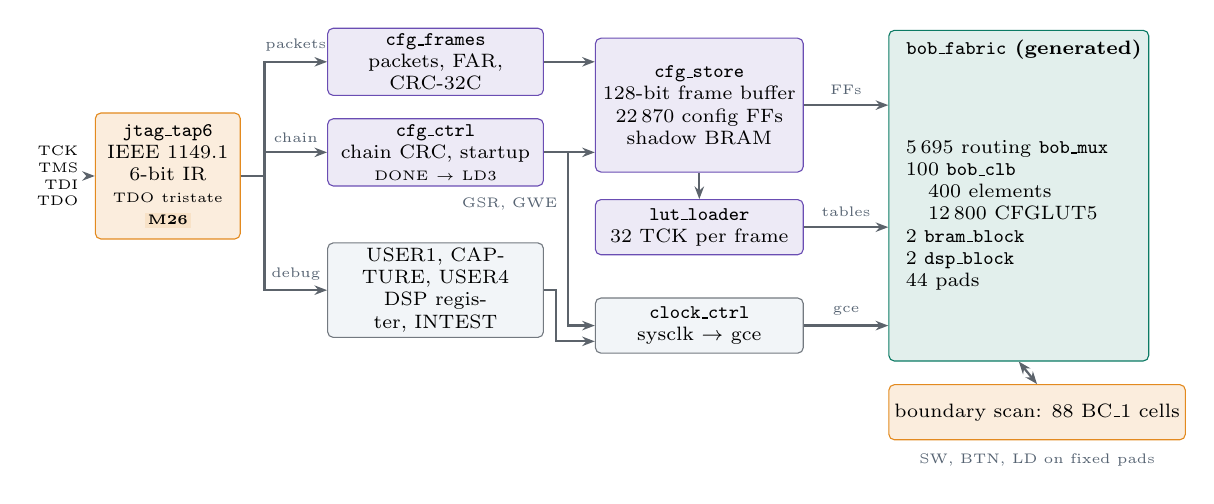
\begin{tikzpicture}[font=\scriptsize]
    \node[font=\tiny, align=right] (pins) at (-0.25,3.0) {TCK\\TMS\\TDI\\TDO};
    \node[hot, text width=17mm, minimum height=16mm] (tap) at (1.15,3.0) {\texttt{jtag\_tap6}\\IEEE 1149.1\\6-bit IR\\\tiny TDO tristate \mtag{M26}};
    \node[cfg, text width=26mm] (frm) at (4.55,4.45) {\texttt{cfg\_frames}\\packets, FAR, CRC-32C};
    \node[cfg, text width=26mm] (ctl) at (4.55,3.3) {\texttt{cfg\_ctrl}\\chain CRC, startup\\\tiny DONE $\rightarrow$ LD3};
    \node[blk, text width=26mm] (dbg) at (4.55,1.55) {USER1, CAPTURE, USER4\\DSP register, INTEST};
    \node[cfg, text width=25mm, minimum height=17mm] (st) at (7.9,3.9) {\texttt{cfg\_store}\\128-bit frame buffer\\22\,870 config FFs\\shadow BRAM};
    \node[cfg, text width=25mm] (ld) at (7.9,2.35) {\texttt{lut\_loader}\\32 TCK per frame};
    \node[blk, text width=25mm] (ck) at (7.9,1.1) {\texttt{clock\_ctrl}\\sysclk $\rightarrow$ gce};
    \node[acc, minimum width=33mm, minimum height=42mm, anchor=west] (fab) at (10.3,2.75) {};
    \node[anchor=north west, font=\scriptsize\bfseries] at (fab.north west) {\ \texttt{bob\_fabric} (generated)};
    \node[anchor=west, font=\scriptsize, align=left] at ($(fab.west)+(0.1,-0.25)$) {5\,695 routing \texttt{bob\_mux}\\100 \texttt{bob\_clb}\\\quad 400 elements\\\quad 12\,800 CFGLUT5\\2 \texttt{bram\_block}\\2 \texttt{dsp\_block}\\44 pads};
    \node[hot, minimum width=33mm, anchor=west] (bsc) at (10.3,0.0) {boundary scan: 88 BC\_1 cells};
    \node[lbl, below=0.5mm of bsc] {SW, BTN, LD on fixed pads};
    \draw[arr] (pins) -- (tap);
    \draw[arr] (tap.east) -- ++(0.3,0) |- node[pos=0.75, above, lbl]{packets} (frm.west);
    \draw[arr] (tap.east) -- ++(0.3,0) |- node[pos=0.75, above, lbl]{chain} (ctl.west);
    \draw[arr] (tap.east) -- ++(0.3,0) |- node[pos=0.75, above, lbl]{debug} (dbg.west);
    \draw[arr] (frm.east) -- (st.west |- frm.east);
    \draw[arr] (ctl.east) -- (st.west |- ctl.east);
    \draw[arr] (ctl.east) -- ++(0.3,0) |- node[pos=0.15, left, lbl]{GSR, GWE} (ck.west);
    \draw[arr] (dbg.east) -- ++(0.15,0) |- ($(ck.west)+(0,-0.2)$);
    \draw[arr] (st) -- (ld);
    \draw[arr] (st.east) -- node[above, lbl]{FFs} (fab.west |- st.east);
    \draw[arr] (ld.east) -- node[above, lbl]{tables} (fab.west |- ld.east);
    \draw[arr] (ck.east) -- node[above, lbl]{gce} (fab.west |- ck.east);
    \draw[arr2] (bsc.north) -- (fab.south);
  \end{tikzpicture}
  \vspace{1mm}

  \small Violet: a small UG470-style controller. Teal: the generated fabric. Every fabric register runs on sysclk and is \emph{enabled} by \texttt{gce}, so holding \texttt{gce} freezes the whole design.
\end{frame}

% =============================================================================
\begin{frame}{The device at M26}
  \begin{columns}[c]
    \column{0.5\textwidth}
    \centering
    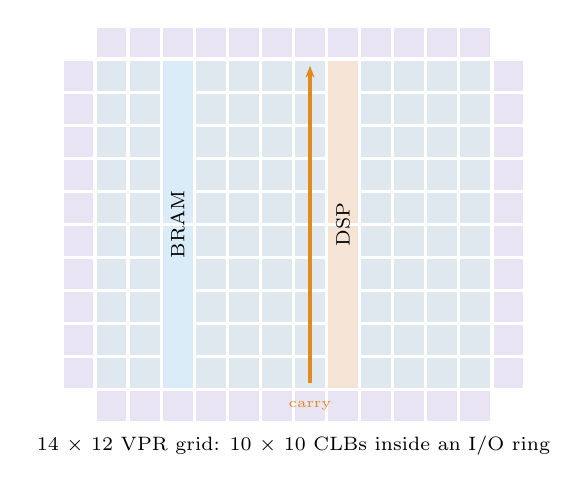
\begin{tikzpicture}[x=4.2mm,y=4.2mm]
      \foreach \x in {1,...,12} { \fill[bobio] (\x+0.05,0.05) rectangle (\x+0.95,0.95); \fill[bobio] (\x+0.05,11.05) rectangle (\x+0.95,11.95); }
      \foreach \y in {1,...,10} { \fill[bobio] (0.05,\y+0.05) rectangle (0.95,\y+0.95); \fill[bobio] (13.05,\y+0.05) rectangle (13.95,\y+0.95); }
      \foreach \x in {1,2,4,5,6,7,9,10,11,12} \foreach \y in {1,...,10}
        { \fill[bobclb] (\x+0.05,\y+0.05) rectangle (\x+0.95,\y+0.95); }
      \fill[bobbram] (3.05,1.05) rectangle (3.95,5.95); \fill[bobbram] (3.05,6.05) rectangle (3.95,10.95);
      \fill[bobdsp] (8.05,1.05) rectangle (8.95,5.95); \fill[bobdsp] (8.05,6.05) rectangle (8.95,10.95);
      \node[font=\scriptsize, rotate=90] at (3.5,6) {BRAM};
      \node[font=\scriptsize, rotate=90] at (8.5,6) {DSP};
      \draw[bobamber, very thick, -{Stealth[length=1.5mm]}] (7.5,1.2) -- (7.5,10.8);
      \node[font=\tiny, color=bobamber] at (7.5,0.5) {carry};
      \node[font=\scriptsize] at (7,-0.7) {14 $\times$ 12 VPR grid: 10 $\times$ 10 CLBs inside an I/O ring};
    \end{tikzpicture}
    \column{0.48\textwidth}
    \footnotesize
    \renewcommand{\arraystretch}{1.15}
    \begin{tabular}{@{}ll@{}}
      \toprule
      CLBs & 100 $\times$ 4 elements = \textbf{400 LUT6} \\
      Element & LUT6 (fracturable), carry, 2 FFs \\
      CLB & N 4, I 16, O 8, 439 config bits \\
      BRAM & 2 $\times$ 1024 $\times$ 18, true dual port \\
      DSP & 2 slices, 25 $\times$ 18, P48, cascade \\
      Routing & L4, W 36, Wilton $F_s$ 3, fc 0.10 \\
      Muxes & 5\,695 routing + 2\,400 crossbar \\
      Pads & 44, with 88 boundary-scan cells \\
      Config & \textbf{532 frames = 68\,096 bits} \\
      IDCODE & \texttt{0x0B026093} (M26) \\
      \bottomrule
    \end{tabular}
    \vspace{2mm}

    \src{Hard-block columns are 5 rows tall. Every number here lives once, in \texttt{device.py}.}
  \end{columns}
\end{frame}

% =============================================================================
\begin{frame}{The logic element (\texttt{ble.sv})}
  \centering
  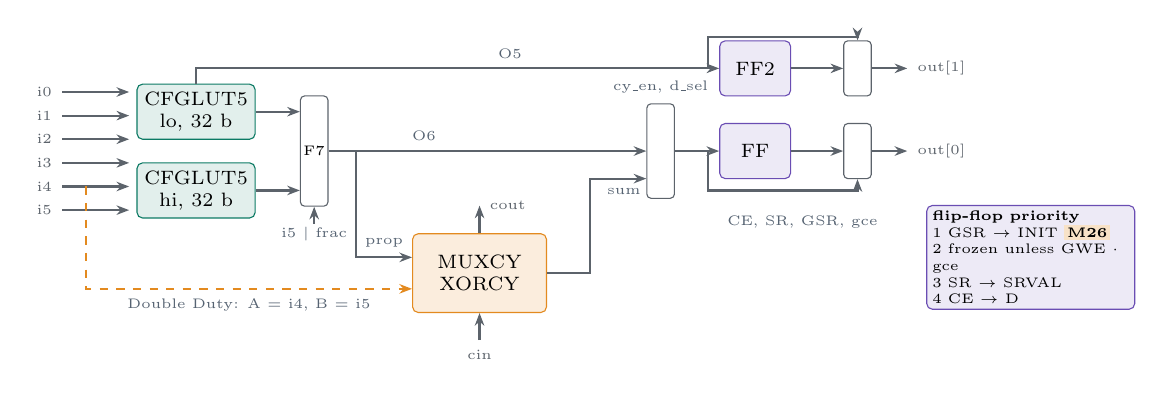
\begin{tikzpicture}[font=\scriptsize]
    \foreach \i/\y in {0/3.0,1/2.7,2/2.4,3/2.1,4/1.8,5/1.5} { \draw[arr] (0,\y) node[left,font=\tiny]{i\i} -- (0.85,\y); }
    \node[acc, minimum width=15mm] (lo) at (1.7,2.75) {CFGLUT5\\lo, 32 b};
    \node[acc, minimum width=15mm] (hi) at (1.7,1.75) {CFGLUT5\\hi, 32 b};
    \node[mx, minimum height=14mm] (f7) at (3.2,2.25) {F7};
    \draw[arr] (lo.east) -- (f7.west |- lo.east);
    \draw[arr] (hi.east) -- (f7.west |- hi.east);
    \node[lbl] at (3.2,1.2) {i5 $|$ frac};
    \draw[arr] (3.2,1.33) -- (f7.south);
    \node[hot, minimum width=17mm, minimum height=10mm] (cy) at (5.3,0.7) {MUXCY\\XORCY};
    \draw[arr] (5.3,-0.15) node[below,font=\tiny]{cin} -- (cy.south);
    \draw[arr] (cy.north) -- ++(0,0.35) node[right,font=\tiny]{cout};
    \draw[arr] (f7.east) -- ++(0.35,0) |- node[pos=0.75,above,lbl]{prop} ($(cy.west)+(0,0.2)$);
    \draw[bobamber, thick, dashed, -{Stealth[length=1.6mm]}] (0.3,1.8) |- node[pos=0.75,below,lbl]{Double Duty: A = i4, B = i5} ($(cy.west)+(0,-0.2)$);
    \node[mx, minimum height=12mm] (dm) at (7.6,2.25) {};
    \node[lbl, above=0mm of dm] {cy\_en, d\_sel};
    \draw[arr] (f7.east) -- node[pos=0.3,above,lbl]{O6} (dm.west |- f7.east);
    \draw[arr] (cy.east) -- ++(0.55,0) |- node[pos=0.8,below,lbl]{sum} ($(dm.west)+(0,-0.35)$);
    \node[cfg, minimum width=9mm] (ff1) at (8.8,2.25) {FF};
    \node[cfg, minimum width=9mm] (ff2) at (8.8,3.3) {FF2};
    \draw[arr] (dm) -- (ff1);
    \draw[arr] (lo.north) |- node[pos=0.8,above,lbl]{O5} (ff2.west);
    \node[mx] (om1) at (10.1,2.25) {};
    \node[mx] (om2) at (10.1,3.3) {};
    \draw[arr] (ff1) -- (om1);  \draw[arr] (ff2) -- (om2);
    \draw[arr] (8.2,2.25) -- ++(0,-0.5) -| (om1.south);
    \draw[arr] (8.2,3.3) -- ++(0,0.4) -| (om2.north);
    \draw[arr] (om1.east) -- ++(0.45,0) node[right,font=\tiny]{out[0]};
    \draw[arr] (om2.east) -- ++(0.45,0) node[right,font=\tiny]{out[1]};
    \node[lbl] at (9.4,1.35) {CE, SR, GSR, gce};
    \node[cfg, text width=25mm, align=left, font=\tiny] at (12.3,0.9) {\textbf{flip-flop priority}\\1\ GSR $\rightarrow$ INIT \mtag{M26}\\2\ frozen unless GWE $\cdot$ gce\\3\ SR $\rightarrow$ SRVAL\\4\ CE $\rightarrow$ D};
  \end{tikzpicture}
  \vspace{1mm}

  \scriptsize
  \begin{columns}[T]
    \column{0.5\textwidth}
    \begin{itemize}
      \item LUT6 = two host \textbf{CFGLUT5}s + MUXF7; with \texttt{frac}: two LUT5s (O6, O5) on 5 shared inputs
      \item Carry after UG474: MUXCY, XORCY
      \item \textbf{Double Duty} (Pun et al., FPL 2025): the adder reads i4, i5 directly, the LUT stays free for out[1]
    \end{itemize}
    \column{0.47\textwidth}
    \begin{itemize}
      \item Two FFs with FDRE/FDSE semantics; M26 splits INIT from SRVAL, as UG474 does
      \item Per element: 64 INIT bits, \textbf{15 flags}, 6 crossbar selects of 5 bits
      \item Checked by \texttt{tb\_clb} against \texttt{model.py}, at K = 6 and K = 4
    \end{itemize}
  \end{columns}
\end{frame}

% =============================================================================
\begin{frame}{The CLB: four elements behind a full crossbar}
  \begin{columns}[c]
    \column{0.55\textwidth}
    \centering
    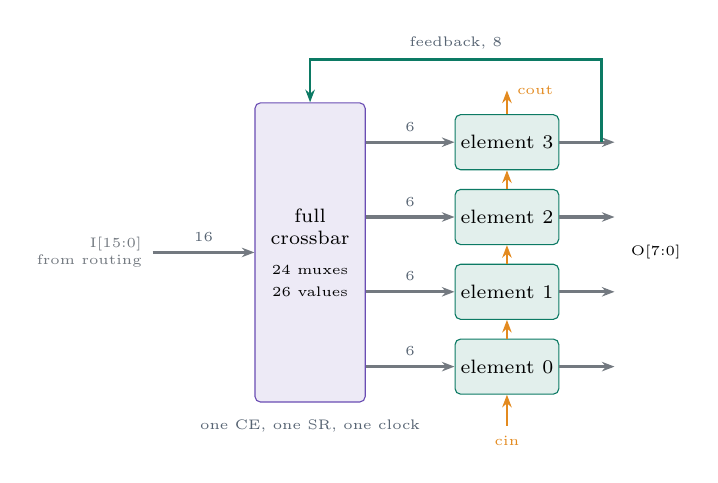
\begin{tikzpicture}[font=\scriptsize]
      \node[cfg, minimum width=14mm, minimum height=38mm] (xb) at (1.6,1.85) {full\\crossbar\\[1mm]\tiny 24 muxes\\\tiny 26 values};
      \foreach \e/\y in {0/0.4,1/1.35,2/2.3,3/3.25} {
        \node[acc, minimum width=13mm] (e\e) at (4.1,\y) {element \e};
        \draw[bus] (xb.east |- e\e.west) -- node[above,lbl]{6} (e\e.west);
        \draw[bus] (e\e.east) -- ++(0.7,0);
      }
      \draw[bus] (-0.4,1.85) node[left,font=\tiny,align=right]{I[15:0]\\from routing} -- node[above,lbl]{16} (xb.west);
      \node[font=\tiny, anchor=west] at (5.55,1.85) {O[7:0]};
      \draw[arr, bobteal] (5.3,3.25) -- (5.3,4.3) -| node[pos=0.25,above,lbl]{feedback, 8} (xb.north);
      \draw[arr, bobamber] (4.1,-0.35) node[below,font=\tiny]{cin} -- (e0.south);
      \foreach \a/\b in {0/1,1/2,2/3} \draw[arr, bobamber] (e\a.north) -- (e\b.south);
      \draw[arr, bobamber] (e3.north) -- ++(0,0.3) node[right,font=\tiny]{cout};
      \node[lbl] at (1.6,-0.35) {one CE, one SR, one clock};
    \end{tikzpicture}
    \column{0.43\textwidth}
    \footnotesize
    \begin{itemize}
      \item After OpenFPGA's \texttt{k6\_frac\_N10}; \textbf{N = 4} with a full crossbar won a measured sweep (N 4, 6, 8, 10)
      \item Each element input picks one of 16 CLB inputs, 8 element outputs, const0, const1
      \item Carry: e0 $\rightarrow$ e3, then the CLB above
    \end{itemize}
    \vspace{1mm}
    \centering
    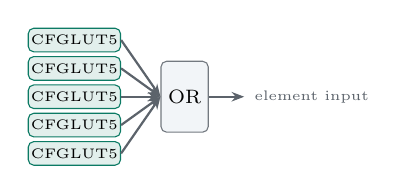
\begin{tikzpicture}[font=\tiny]
      \foreach \k in {0,...,4} \node[acc, minimum width=9mm, minimum height=3mm, inner sep=1pt, font=\tiny] (l\k) at (0,-\k*0.36) {CFGLUT5};
      \node[blk, minimum width=6mm, minimum height=9mm] (or) at (1.4,-0.72) {OR};
      \foreach \k in {0,...,4} \draw[arr] (l\k.east) -- (or.west);
      \draw[arr] (or.east) -- ++(0.45,0) node[right]{element input};
    \end{tikzpicture}

    \src{One crossbar mux (\texttt{lxor.v}): five leaves and a fixed OR; an unselected leaf holds zeros. 128 CFGLUT5 per CLB.}
  \end{columns}
\end{frame}

% =============================================================================
\begin{frame}{Routing: generated from VPR's own rr graph}
  \begin{columns}[c]
    \column{0.48\textwidth}
    \centering
    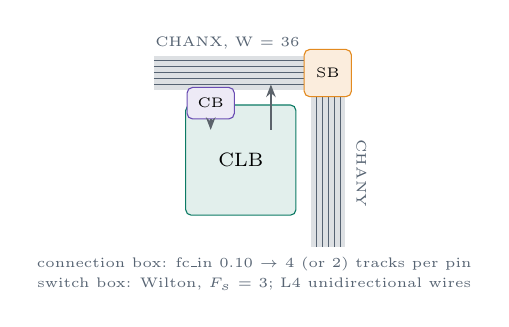
\begin{tikzpicture}[font=\scriptsize, x=0.85cm, y=0.85cm]
      \node[acc, minimum width=14mm, minimum height=14mm] (clb) at (0,0) {CLB};
      \fill[bobmute!20] (-1.3,1.05) rectangle (1.05,1.55);
      \fill[bobmute!20] (1.05,-1.3) rectangle (1.55,1.05);
      \foreach \tr in {1.13,1.22,1.31,1.40,1.49} \draw[bobmute] (-1.3,\tr) -- (1.05,\tr);
      \foreach \tr in {1.13,1.22,1.31,1.40,1.49} \draw[bobmute] (\tr,-1.3) -- (\tr,1.05);
      \node[hot, minimum width=6mm, minimum height=6mm, font=\tiny] (sb) at (1.3,1.3) {SB};
      \node[lbl] at (-0.2,1.75) {CHANX, W = 36};
      \node[lbl, rotate=-90] at (1.8,-0.2) {CHANY};
      \node[cfg, minimum width=6mm, minimum height=4mm, font=\tiny] (cb) at (-0.45,0.85) {CB};
      \draw[arr] (cb.south) -- (-0.45,0.45);
      \draw[arr] (0.45,0.45) -- (0.45,1.13);
      \node[lbl] at (0.2,-1.55) {connection box: fc\_in 0.10 $\rightarrow$ 4 (or 2) tracks per pin};
      \node[lbl] at (0.2,-1.85) {switch box: Wilton, $F_s$ = 3; L4 unidirectional wires};
    \end{tikzpicture}

    \vspace{2mm}
    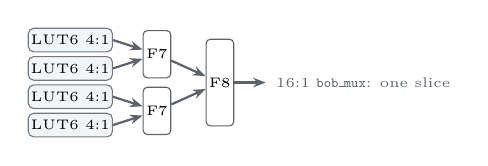
\begin{tikzpicture}[font=\tiny]
      \foreach \k in {0,...,3} \node[blk, minimum width=9mm, minimum height=3mm, inner sep=1pt, font=\tiny] (q\k) at (0,-\k*0.36) {LUT6 4:1};
      \node[mx, minimum height=6mm] (m7a) at (1.1,-0.18) {F7};
      \node[mx, minimum height=6mm] (m7b) at (1.1,-0.9) {F7};
      \node[mx, minimum height=11mm] (m8) at (1.9,-0.54) {F8};
      \draw[arr] (q0.east) -- (m7a); \draw[arr] (q1.east) -- (m7a);
      \draw[arr] (q2.east) -- (m7b); \draw[arr] (q3.east) -- (m7b);
      \draw[arr] (m7a) -- (m8); \draw[arr] (m7b) -- (m8);
      \draw[arr] (m8.east) -- ++(0.4,0) node[right]{16:1 \texttt{bob\_mux}: one slice};
    \end{tikzpicture}
    \column{0.5\textwidth}
    \footnotesize
    \begin{itemize}
      \item VPR builds the \textbf{routing-resource graph}: every wire and pin a node, every switch an edge
      \item \texttt{fabric\_gen.py} (the OpenFPGA method): \alert{every node with fan-in is a mux}; its select bits are configuration bits
      \item Value 0 = const0: an all-zero configuration is a dark, loop-free fabric
    \end{itemize}
    \vspace{2mm}
    \centering
    \scriptsize
    \begin{tabular}{@{}lrr@{}}
      \toprule
      mux kind (inputs) & muxes & select bits \\
      \midrule
      IPIN, connection box (4 or 2) & 2\,220 & 6\,296 \\
      CHANX, CHANY, switch box (1--13) & 3\,475 & 10\,486 \\
      crossbar, in the CLBs (24 + 2 const) & 2\,400 & 12\,000 \\
      \bottomrule
    \end{tabular}
  \end{columns}
\end{frame}

% =============================================================================
\begin{frame}{The hard blocks: BRAM (after UG473) and DSP (after UG479)}
  \begin{columns}[T]
    \column{0.47\textwidth}
    \centering
    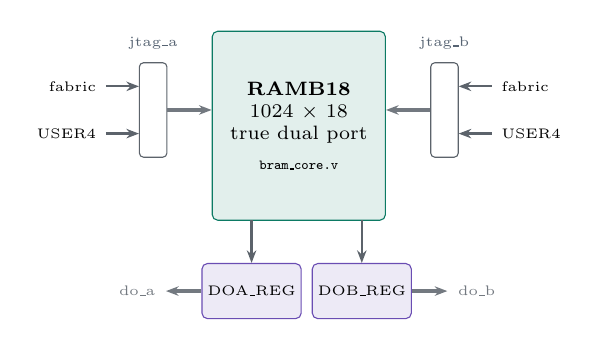
\begin{tikzpicture}[font=\scriptsize]
      \node[acc, minimum width=22mm, minimum height=24mm] (core) at (3.1,1.9) {\textbf{RAMB18}\\1024 $\times$ 18\\true dual port\\[1mm]\tiny\texttt{bram\_core.v}};
      \node[mx, minimum height=12mm] (ma) at (1.25,2.1) {};
      \node[mx, minimum height=12mm] (mb) at (4.95,2.1) {};
      \node[font=\tiny, anchor=east] at (0.65,2.4) {fabric};
      \node[font=\tiny, anchor=east] at (0.65,1.8) {USER4};
      \node[font=\tiny, anchor=west] at (5.55,2.4) {fabric};
      \node[font=\tiny, anchor=west] at (5.55,1.8) {USER4};
      \draw[arr] (0.65,2.4) -- (1.07,2.4);
      \draw[arr] (0.65,1.8) -- (1.07,1.8);
      \draw[arr] (5.55,2.4) -- (5.13,2.4);
      \draw[arr] (5.55,1.8) -- (5.13,1.8);
      \draw[bus] (ma.east) -- (core.west |- ma.east);
      \draw[bus] (mb.west) -- (core.east |- mb.west);
      \node[cfg, font=\tiny] (ra) at (2.5,-0.2) {DOA\_REG};
      \node[cfg, font=\tiny] (rb) at (3.9,-0.2) {DOB\_REG};
      \draw[arr] (2.5,0.7) -- (ra.north);
      \draw[arr] (3.9,0.7) -- (rb.north);
      \draw[bus] (ra.west) -- ++(-0.45,0) node[left, font=\tiny]{do\_a};
      \draw[bus] (rb.east) -- ++(0.45,0) node[right, font=\tiny]{do\_b};
      \node[lbl] at (1.25,2.95) {jtag\_a};
      \node[lbl] at (4.95,2.95) {jtag\_b};
    \end{tikzpicture}
    \scriptsize
    \begin{itemize}
      \item \textbf{8 config bits}: write mode per port (WRITE\_FIRST, READ\_FIRST, NO\_CHANGE), output register, pins from JTAG
      \item Inference template $\Rightarrow$ a real host RAMB18
      \item \textbf{Contents are not configuration}: FAR block type 001, under the same CRC; survive JPROGRAM
    \end{itemize}
    \column{0.51\textwidth}
    \centering
    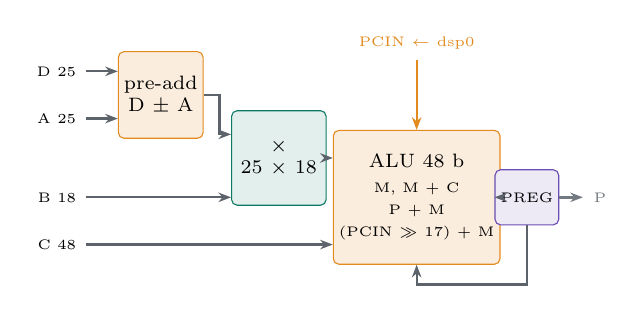
\begin{tikzpicture}[font=\scriptsize]
      \node[font=\tiny, anchor=east] (d) at (0,2.6) {D 25};
      \node[font=\tiny, anchor=east] (a) at (0,2.0) {A 25};
      \node[font=\tiny, anchor=east] (b) at (0,1.0) {B 18};
      \node[font=\tiny, anchor=east] (c) at (0,0.4) {C 48};
      \node[hot, minimum width=10mm, minimum height=11mm] (pre) at (0.95,2.3) {pre-add\\D $\pm$ A};
      \draw[arr] (d) -- (pre.west |- d); \draw[arr] (a) -- (pre.west |- a);
      \node[acc, minimum width=12mm, minimum height=12mm] (mul) at (2.45,1.5) {$\times$\\25 $\times$ 18};
      \draw[arr] (pre.east) -- ++(0.2,0) |- ($(mul.west)+(0,0.3)$);
      \draw[arr] (b) -- ($(mul.west)+(0,-0.5)$);
      \node[hot, minimum width=15mm, minimum height=17mm] (alu) at (4.2,1.0) {ALU 48 b\\[1pt]\tiny M, M + C\\\tiny P + M\\\tiny (PCIN $\gg$ 17) + M};
      \draw[arr] (mul.east) -- ($(alu.west)+(0,0.5)$);
      \draw[arr] (c) -- (alu.west |- c);
      \node[cfg, font=\tiny] (pr) at (5.6,1.0) {PREG};
      \draw[arr] (alu) -- (pr);
      \draw[bus] (pr.east) -- ++(0.3,0) node[right,font=\tiny]{P};
      \draw[arr] (pr.south) -- ++(0,-0.75) -| (alu.south);
      \draw[arr, bobamber] (4.2,2.75) node[above,font=\tiny]{PCIN $\leftarrow$ dsp0} -- (alu.north);
    \end{tikzpicture}
    \scriptsize
    \begin{itemize}
      \item \textbf{16 config bits}: opmode, pre-adder use/subtract, A/B/C/D/M/P registers, JTAG drive
      \item Static opmodes instead of dynamic OPMODE pins: no routing spent on control; the \textbf{cascade} kept for filters
      \item yosys maps \texttt{*} with \texttt{mul2dsp}; \texttt{fir.v} uses both slices
    \end{itemize}
  \end{columns}
\end{frame}

% =============================================================================
\begin{frame}{Mapping the guest onto the XC7Z020 (the M26 build)}
  \begin{columns}[c]
    \column{0.54\textwidth}
    \scriptsize
    \renewcommand{\arraystretch}{1.25}
    \begin{tabular}{@{}lcl@{}}
      \toprule
      \textbf{guest resource} & & \textbf{host primitives} \\
      \midrule
      LUT6, 64-bit table & $\rightarrow$ & 2 CFGLUT5 + MUXF7 \\
      crossbar mux, 26 values & $\rightarrow$ & 5 CFGLUT5 + OR \\
      routing mux, $\leq$ 16:1 & $\rightarrow$ & LUT6 leaves + MUXF7/F8 \\
      flags, routing selects & $\rightarrow$ & 22\,870 flip-flops \\
      user flip-flop & $\rightarrow$ & FDRE, CE = gce \\
      BRAM 1K $\times$ 18 & $\rightarrow$ & RAMB18E1, inferred \\
      DSP slice & $\rightarrow$ & DSP48E1 \\
      readback copy & $\rightarrow$ & shadow BRAM \\
      \bottomrule
    \end{tabular}
    \vspace{2mm}

    \src{A CFGLUT5 is AMD's LUT5 whose table is shifted in (UG953): the guest's truth tables and crossbar choices live \emph{in} host LUTRAM, as in ZUMA (FCCM 2012).}
    \column{0.44\textwidth}
    \centering
    \textbf{\small Share of the XC7Z020 used}\\[2mm]
    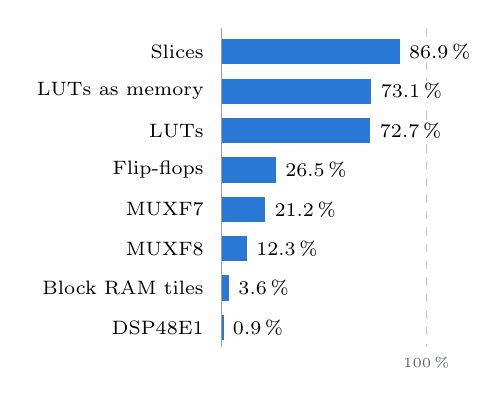
\begin{tikzpicture}[font=\scriptsize, x=0.26mm]
      \draw[bobmute!35, dashed] (100,0.3) -- (100,-3.75) node[below, lbl]{100\,\%};
      \draw[bobmute!60] (0,0.3) -- (0,-3.75);
      \foreach \y/\nm/\val in {0/Slices/86.9, 1/LUTs as memory/73.1, 2/LUTs/72.7, 3/Flip-flops/26.5, 4/MUXF7/21.2, 5/MUXF8/12.3, 6/Block RAM tiles/3.6, 7/DSP48E1/0.9} {
        \node[anchor=east, font=\scriptsize] at (-4,{-\y*0.5}) {\nm};
        \fill[vizA] (0,{-\y*0.5-0.16}) rectangle (\val,{-\y*0.5+0.16});
        \node[anchor=west, font=\scriptsize, fill=white, inner sep=1pt] at (\val+3,{-\y*0.5}) {\val\,\%};
      }
    \end{tikzpicture}
  \end{columns}
  \vspace{2mm}
  \centering
  \small 38\,676 LUTs $\cdot$ 28\,186 FFs $\cdot$ WNS +0.287 ns (sysclk 125 MHz), +479.8 ns (TCK 1 MHz)\\
  \alert{Slices 86.9\,\%: 10 $\times$ 10 CLBs is this CLB's ceiling on the XC7Z020.}
\end{frame}

% =============================================================================
\begin{frame}{Why the RTL looks the way it does: host LUTs per guest LUT}
  \begin{columns}[c]
    \column{0.52\textwidth}
    \centering
    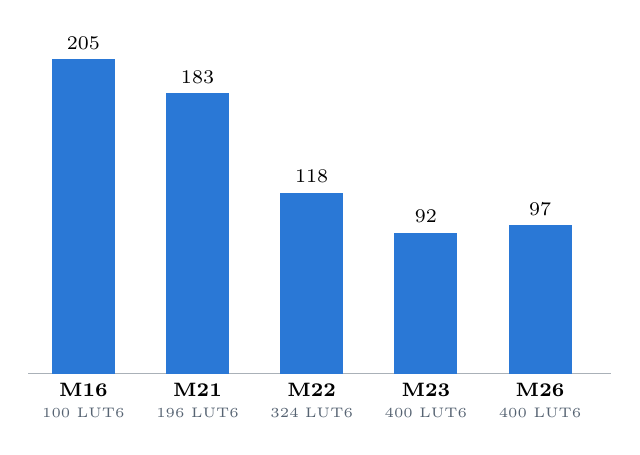
\begin{tikzpicture}[font=\scriptsize, y=0.195mm]
      \draw[bobmute!50] (-0.2,0) -- (7.2,0);
      \foreach \i/\m/\val/\gl in {0/M16/205/100, 1/M21/183/196, 2/M22/118/324, 3/M23/92/400, 4/M26/97/400} {
        \fill[vizA] ({\i*1.45+0.1},0) rectangle ({\i*1.45+0.9},\val);
        \node[anchor=south, font=\scriptsize] at ({\i*1.45+0.5},\val) {\val};
        \node[anchor=north, font=\scriptsize\bfseries] at ({\i*1.45+0.5},0) {\m};
        \node[anchor=north, lbl] at ({\i*1.45+0.5},-16) {\gl\ LUT6};
      }
    \end{tikzpicture}

    \src{Vivado's host LUT count divided by the guest's LUT6 count, per build. Below each bar: the guest's size.}
    \column{0.46\textwidth}
    \scriptsize
    \begin{tabular}{@{}L{10mm}L{50mm}@{}}
      \toprule
      \textbf{M21} & the cluster CLB (N 4, full crossbar); readback from a shadow BRAM instead of a 256:1 mux: $-$11.8k LUTs \\
      \textbf{M22} & truth tables and crossbar in CFGLUT5: a CLB 469 $\rightarrow$ 193 host LUTs (yosys) \\
      \textbf{M23} & crossbar root = a fixed OR (152 $\rightarrow$ 128 CFGLUT5 per CLB); routing muxes as LUT6 + MUXF7 + MUXF8 \\
      \textbf{M24--26} & features on the same grid: Double Duty, GRESTORE, INIT bits \\
      \bottomrule
    \end{tabular}
    \vspace{2mm}

    Every step was \textbf{measured before it was built}: \texttt{sweep.py}, \texttt{gridsweep.py}, \texttt{synth\_estimate.sh}.
  \end{columns}
\end{frame}

% =============================================================================
\begin{frame}{The user clock: an enable, not a clock (\texttt{clock\_ctrl.v})}
  \centering
  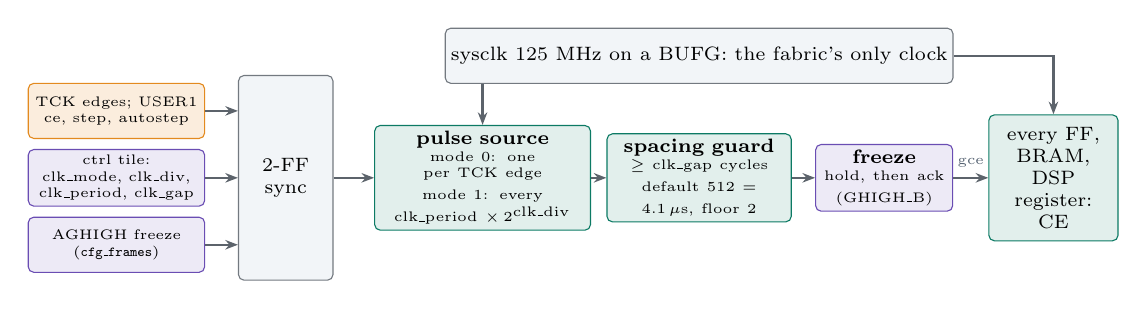
\begin{tikzpicture}[font=\scriptsize]
    \node[hot, text width=21mm, font=\tiny] (in1) at (1.15,3.05) {TCK edges; USER1 ce, step, autostep};
    \node[cfg, text width=21mm, font=\tiny] (in2) at (1.15,2.2) {ctrl tile: clk\_mode, clk\_div, clk\_period, clk\_gap};
    \node[cfg, text width=21mm, font=\tiny] (in3) at (1.15,1.35) {AGHIGH freeze (\texttt{cfg\_frames})};
    \node[blk, minimum width=12mm, minimum height=26mm] (sy) at (3.3,2.2) {2-FF\\sync};
    \node[acc, text width=26mm] (gen) at (5.8,2.2) {\textbf{pulse source}\\\tiny mode 0: one per TCK edge\\\tiny mode 1: every clk\_period $\times\,2^{\mathrm{clk\_div}}$};
    \node[acc, text width=22mm] (gap) at (8.55,2.2) {\textbf{spacing guard}\\\tiny $\geq$ clk\_gap cycles\\\tiny default 512 = 4.1\,$\mu$s, floor 2};
    \node[cfg, text width=16mm] (frz) at (10.9,2.2) {\textbf{freeze}\\\tiny hold, then ack\\\tiny (GHIGH\_B)};
    \node[acc, text width=15mm, minimum height=16mm] (fab) at (13.05,2.2) {every FF, BRAM, DSP register: CE};
    \node[blk, minimum width=60mm] (clk) at (8.55,3.75) {sysclk 125 MHz on a BUFG: the fabric's only clock};
    \draw[arr] (in1.east) -- (sy.west |- in1.east);
    \draw[arr] (in2.east) -- (sy.west |- in2.east);
    \draw[arr] (in3.east) -- (sy.west |- in3.east);
    \draw[arr] (sy) -- (gen); \draw[arr] (gen) -- (gap); \draw[arr] (gap) -- (frz);
    \draw[arr] (frz) -- node[above, lbl]{gce} (fab);
    \draw[arr] (clk.east) -| (fab.north);
    \draw[arr] (clk.south -| gen.north) -- (gen.north);
  \end{tikzpicture}
  \vspace{2mm}

  \begin{columns}[T]
    \column{0.5\textwidth}
    \small\textbf{Why an enable}
    \scriptsize
    \begin{itemize}
      \item One real clock: nothing derived or gated (UG949)
      \item Cycle-exact: one user clock per scan, board vs \texttt{model.py} every clock
      \item Freeze = hold \texttt{gce}: partial reload and snapshots keep all state
    \end{itemize}
    \column{0.46\textwidth}
    \small\textbf{Per design}
    \scriptsize
    \begin{itemize}
      \item \texttt{timing.py} sets \texttt{clk\_gap} from the design's own path
      \item \texttt{counter}: 12.9 ns $\times$ 2 $\rightarrow$ 4 cycles $\rightarrow$ \textbf{31.25 MHz}
      \item Hardware floor: 2 cycles = 62.5 MHz
    \end{itemize}
  \end{columns}
\end{frame}

% =============================================================================
\begin{frame}{JTAG: the only way in (\texttt{jtag\_tap6.v})}
  \begin{columns}[c]
    \column{0.6\textwidth}
    \centering
    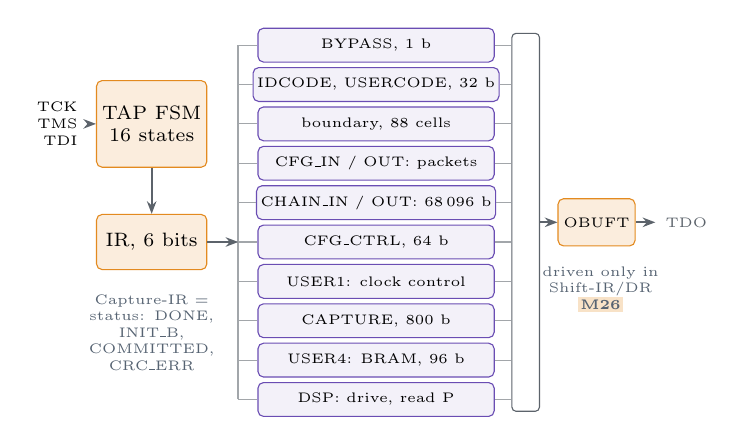
\begin{tikzpicture}[font=\scriptsize]
      \node[font=\tiny, align=right] (pins) at (-0.3,3.6) {TCK\\TMS\\TDI};
      \node[hot, minimum width=14mm, minimum height=11mm] (fsm) at (0.9,3.6) {TAP FSM\\16 states};
      \node[hot, minimum width=14mm] (ir) at (0.9,2.1) {IR, 6 bits};
      \node[lbl, text width=16mm, align=center] at (0.9,0.95) {Capture-IR = status: DONE, INIT\_B, COMMITTED, CRC\_ERR};
      \draw[arr] (pins) -- (fsm);
      \draw[arr] (fsm) -- (ir);
      \foreach \nm/\y/\tx in {r0/4.6/{BYPASS, 1 b}, r1/4.1/{IDCODE, USERCODE, 32 b}, r2/3.6/{boundary, 88 cells}, r3/3.1/{CFG\_IN / OUT: packets}, r4/2.6/{CHAIN\_IN / OUT: 68\,096 b}, r5/2.1/{CFG\_CTRL, 64 b}, r6/1.6/{USER1: clock control}, r7/1.1/{CAPTURE, 800 b}, r8/0.6/{USER4: BRAM, 96 b}, r9/0.1/{DSP: drive, read P}}
      {
        \node[bx, sm, draw=bobviolet, fill=bobviolet!8, minimum width=30mm] (\nm) at (3.75,\y) {\tx};
        \draw[bobink!40] (2.0,\y) -- (\nm.west);
      }
      \draw[bobink!40, thick] (2.0,0.1) -- (2.0,4.6);
      \draw[arr] (ir.east) -- (2.0,2.1);
      \node[mx, minimum height=48mm] (tm) at (5.65,2.35) {};
      \foreach \nm in {r0,r1,r2,r3,r4,r5,r6,r7,r8,r9} \draw[bobink!40] (\nm.east) -- (tm.west |- \nm.east);
      \node[hot, font=\tiny, minimum height=6mm] (ob) at (6.55,2.35) {OBUFT};
      \draw[arr] (tm) -- (ob);
      \draw[arr] (ob.east) -- ++(0.25,0) node[right, font=\tiny]{TDO};
      \node[lbl, align=center] at (6.6,1.5) {driven only in\\Shift-IR/DR\\\mtag{M26}};
    \end{tikzpicture}
    \column{0.38\textwidth}
    \scriptsize
    \begin{tabular}{@{}ll@{}}
      \toprule
      instruction & code \\
      \midrule
      IDCODE & 001001 \\
      CFG\_IN, CFG\_OUT & 000101, 000100 \\
      JPROGRAM, JSTART & 001011, 001100 \\
      USER1 (clock) & 000010 \\
      USER2 (CFG\_CTRL) & 000011 \\
      USER3 (CAPTURE) & 100010 \\
      USER4 (BRAM) & 100011 \\
      SAMPLE, EXTEST & 000001, 100110 \\
      INTEST$^*$ & 000111 \\
      DSP$^*$ & 101000 \\
      CHAIN\_IN, OUT$^*$ & 110101, 110100 \\
      \bottomrule
    \end{tabular}

    \vspace{1mm}
    \src{AMD 7-series codes where they exist; $^*$ = bob's own. TMS, TDI on the rising edge; TDO and updates on the falling edge.}
  \end{columns}
\end{frame}

% =============================================================================
\section{Configuration}
\begin{frame}{Configuration memory: frames, FAR and where the bits go}
  \centering
  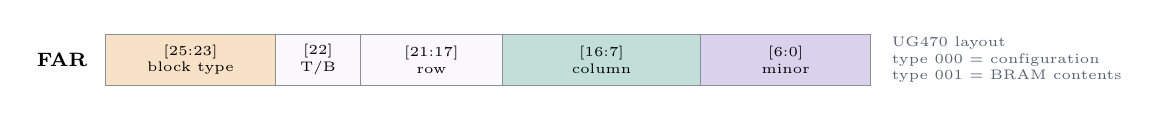
\begin{tikzpicture}[font=\scriptsize, x=3.6mm, y=6.5mm]
    \foreach \lo/\hi/\tx/\col in {0/6/{[25:23]\\block type}/bobamber, 6/9/{[22]\\T/B}/bobio, 9/14/{[21:17]\\row}/bobio, 14/21/{[16:7]\\column}/bobteal, 21/27/{[6:0]\\minor}/bobviolet}
      { \fill[\col!25] (\lo,0) rectangle (\hi,1); \draw[bobink!50] (\lo,0) rectangle (\hi,1); \node[font=\tiny, align=center] at ({(\lo+\hi)/2},0.5) {\tx}; }
    \node[anchor=east, font=\scriptsize\bfseries] at (-0.3,0.5) {FAR};
    \node[anchor=west, font=\tiny, color=bobmute, align=left] at (27.4,0.5) {UG470 layout\\type 000 = configuration\\type 001 = BRAM contents};
  \end{tikzpicture}
  \vspace{3mm}

  \begin{columns}[c]
    \column{0.42\textwidth}
    \centering
    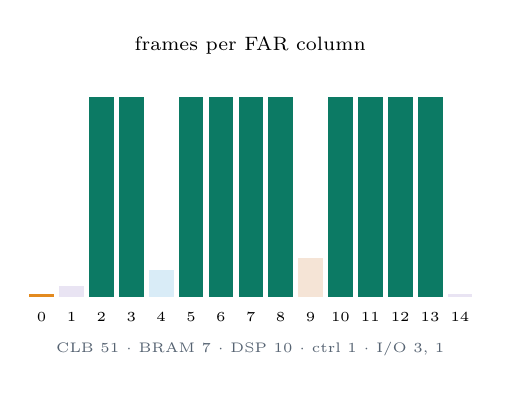
\begin{tikzpicture}[x=3.3mm,y=0.5mm]
      \foreach \cc/\nfr/\col in {0/1/bobamber,1/3/bobio,2/51/bobteal,3/51/bobteal,4/7/bobbram,5/51/bobteal,6/51/bobteal,7/51/bobteal,8/51/bobteal,9/10/bobdsp,10/51/bobteal,11/51/bobteal,12/51/bobteal,13/51/bobteal,14/1/bobio}
        { \fill[\col] (\cc*1.15,0) rectangle (\cc*1.15+0.95,\nfr); \node[font=\tiny] at (\cc*1.15+0.47,-5) {\cc}; }
      \node[font=\scriptsize, align=center] at (8.5,64) {frames per FAR column};
      \node[font=\tiny, color=bobmute] at (8.5,-13) {CLB 51 $\cdot$ BRAM 7 $\cdot$ DSP 10 $\cdot$ ctrl 1 $\cdot$ I/O 3, 1};
    \end{tikzpicture}
    \column{0.56\textwidth}
    \centering
    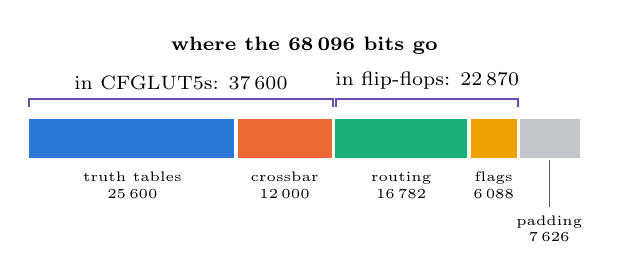
\begin{tikzpicture}[font=\tiny, x=1cm, y=1cm]
      % 68,096 bits over 7.0 cm
      \foreach \a/\b/\col in {0/2.632/vizA, 2.632/3.866/vizB, 3.866/5.591/vizC, 5.591/6.217/vizD, 6.217/7.0/vizN}
        { \fill[\col] (\a,0) rectangle (\b,0.5); }
      \foreach \xx in {2.632,3.866,5.591,6.217} \draw[white, line width=1.2pt] (\xx,-0.01) -- (\xx,0.51);
      \node[anchor=north, align=center] at (1.316,-0.05) {truth tables\\25\,600};
      \node[anchor=north, align=center] at (3.249,-0.05) {crossbar\\12\,000};
      \node[anchor=north, align=center] at (4.729,-0.05) {routing\\16\,782};
      \node[anchor=north, align=center] at (5.904,-0.05) {flags\\6\,088};
      \draw[bobmute] (6.61,-0.02) -- (6.61,-0.62);
      \node[anchor=north, align=center] at (6.61,-0.6) {padding\\7\,626};
      \draw[bobviolet, thick] (0,0.65) -- (0,0.75) -- (3.866,0.75) -- (3.866,0.65);
      \node[anchor=south, font=\scriptsize] at (1.933,0.75) {in CFGLUT5s: 37\,600};
      \draw[bobviolet, thick] (3.9,0.65) -- (3.9,0.75) -- (6.217,0.75) -- (6.217,0.65);
      \node[anchor=south, font=\scriptsize] at (5.06,0.75) {in flip-flops: 22\,870};
      \node[anchor=south, font=\scriptsize\bfseries] at (3.5,1.2) {where the 68\,096 bits go};
    \end{tikzpicture}
  \end{columns}
  \vspace{2mm}

  \small A \textbf{frame} = 4 words = 128 bits, the unit of writing and reading; \textbf{532 frames}, column by column as on 7-series. FAR counts up by itself. The scan chain is all frames end to end.
\end{frame}

% =============================================================================
\begin{frame}{One CLB tile = 5 frames (M26 layout)}
  \centering
  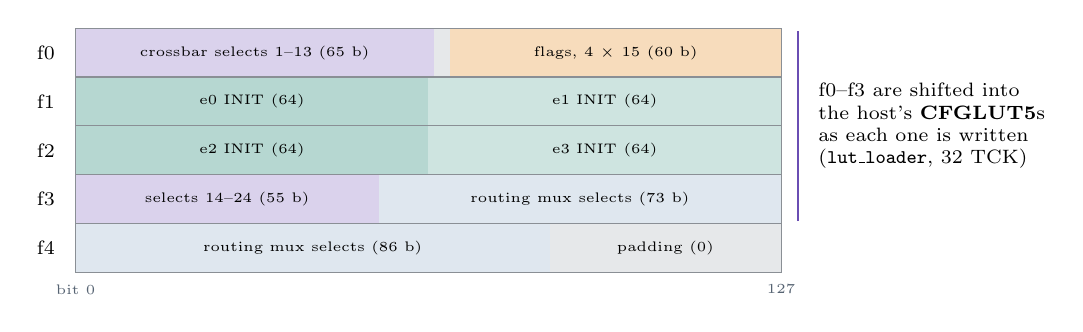
\begin{tikzpicture}[font=\tiny, x=0.7mm, y=6.2mm]
    \node[anchor=east, font=\scriptsize] at (-2,4.5) {f0};
    \fill[bobviolet!25] (0,4) rectangle (65,5); \node at (32.5,4.5) {crossbar selects 1--13 (65 b)};
    \fill[bobmute!15] (65,4) rectangle (68,5);
    \fill[bobamber!30] (68,4) rectangle (128,5); \node at (98,4.5) {flags, 4 $\times$ 15 (60 b)};
    \node[anchor=east, font=\scriptsize] at (-2,3.5) {f1};
    \fill[bobteal!30] (0,3) rectangle (64,4); \node at (32,3.5) {e0 INIT (64)};
    \fill[bobteal!20] (64,3) rectangle (128,4); \node at (96,3.5) {e1 INIT (64)};
    \node[anchor=east, font=\scriptsize] at (-2,2.5) {f2};
    \fill[bobteal!30] (0,2) rectangle (64,3); \node at (32,2.5) {e2 INIT (64)};
    \fill[bobteal!20] (64,2) rectangle (128,3); \node at (96,2.5) {e3 INIT (64)};
    \node[anchor=east, font=\scriptsize] at (-2,1.5) {f3};
    \fill[bobviolet!25] (0,1) rectangle (55,2); \node at (27.5,1.5) {selects 14--24 (55 b)};
    \fill[bobclb] (55,1) rectangle (128,2); \node at (91.5,1.5) {routing mux selects (73 b)};
    \node[anchor=east, font=\scriptsize] at (-2,0.5) {f4};
    \fill[bobclb] (0,0) rectangle (86,1); \node at (43,0.5) {routing mux selects (86 b)};
    \fill[bobmute!15] (86,0) rectangle (128,1); \node at (107,0.5) {padding (0)};
    \foreach \y in {0,1,2,3,4} \draw[bobink!50] (0,\y) rectangle (128,\y+1);
    \node[color=bobmute] at (0,-0.35) {bit 0};
    \node[color=bobmute] at (128,-0.35) {127};
    \draw[bobviolet, thick] (131,1.05) -- (131,4.95);
    \node[anchor=west, font=\scriptsize, align=left] at (133,3) {f0--f3 are shifted into\\the host's \textbf{CFGLUT5}s\\as each one is written\\(\texttt{lut\_loader}, 32 TCK)};
  \end{tikzpicture}
  \vspace{2mm}

  \footnotesize
  \begin{itemize}
    \item Tile \texttt{clb\_x1y1} = chain bits 640--1279 = frames 5--9 (FAR column 2, minors 1--5): 439 CLB bits, then 159 routing bits
    \item Flags and routing selects land in flip-flops; each 5-bit crossbar select is expanded at load time into its five leaf tables (\texttt{lut\_expand.v})
    \item M26 added two flags per element (\texttt{ff\_init}, \texttt{ff2\_init}): 13 $\rightarrow$ 15, still 5 frames per tile
  \end{itemize}
\end{frame}

% =============================================================================
\begin{frame}{The packet stream (after UG470 chapter 5): the counter, sparse}
  \begin{columns}[T]
    \column{0.52\textwidth}
    \ttfamily\scriptsize
    \begin{tabular}{@{}ll@{}}
      FFFFFFFF FFFFFFFF & \sffamily dummy \\
      \textcolor{bobamber}{AA995566} & \textcolor{bobamber}{\sffamily sync word} \\
      30008001 00000007 & \sffamily CMD = RCRC \\
      30018001 \textcolor{bobteal}{0B026093} & \sffamily IDCODE must match \\
      30008001 00000001 & \sffamily CMD = WCFG \\
      30002001 00000080 & \sffamily FAR: column 1, minor 0 \\
      30004008 \sffamily 8 words & \sffamily FDRI: 2 frames \\
      30002001 00000119 & \sffamily FAR: column 2, minor 25 \\
      30004004 00100000 \dots & \sffamily FDRI: holds \texttt{rr6840} \\
      \sffamily \dots\ 24 runs, 30 frames \dots & \\
      30000001 95ADDD48 & \sffamily CRC-32C check \\
      30008001 00000003 & \sffamily LFRM \\
      30008001 00000005 & \sffamily START \\
      30008001 0000000D & \sffamily DESYNC \\
    \end{tabular}

    \vspace{2mm}
    \sffamily\tiny
    \begin{tabular}{@{}ll@{}}
      \toprule
      type 1 & \texttt{[31:29]} = 001, op \texttt{[28:27]}, register \texttt{[17:13]}, count \texttt{[10:0]} \\
      type 2 & \texttt{[31:29]} = 010, op \texttt{[28:27]}, count \texttt{[26:0]} \\
      \bottomrule
    \end{tabular}
    \column{0.46\textwidth}
    \footnotesize
    \begin{itemize}
      \item The parser \alert{hunts} for the sync word bit by bit, then reads 32-bit words: a stream may span any number of JTAG scans
      \item Registers CRC, FAR, FDRI, FDRO, CMD, STAT, IDCODE at 7-series addresses
      \item \textbf{CRC-32C} over \{register, data\} of every write: one wrong bit and START is refused
      \item Frames need WCFG, the right IDCODE and GWE = 0
      \item \textbf{Sparse}: after JPROGRAM only frames holding a 1. \texttt{counter}: \textbf{214 words}, not 2\,154
    \end{itemize}
  \end{columns}
\end{frame}

% =============================================================================
\begin{frame}{The configuration datapath and startup}
  \centering
  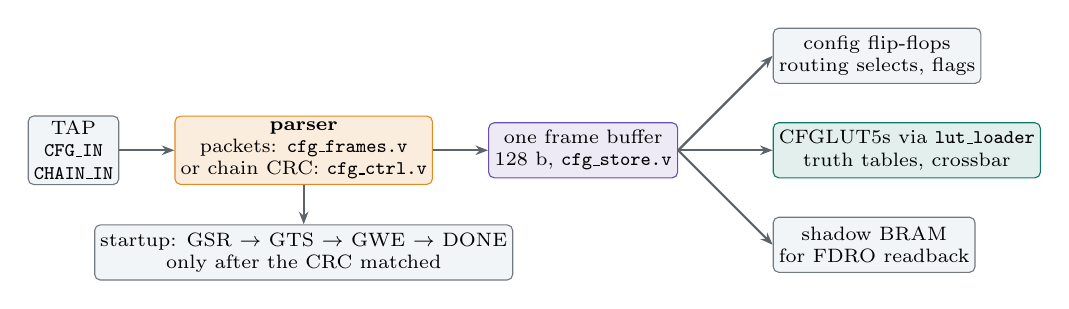
\begin{tikzpicture}[node distance=5mm and 7mm, font=\scriptsize]
    \node[blk] (tap) {TAP\\\texttt{CFG\_IN}\\\texttt{CHAIN\_IN}};
    \node[hot, right=of tap, minimum width=30mm] (par) {\textbf{parser}\\packets: \texttt{cfg\_frames.v}\\or chain CRC: \texttt{cfg\_ctrl.v}};
    \node[blk, below=of par] (ctrl) {startup: GSR $\rightarrow$ GTS $\rightarrow$ GWE $\rightarrow$ DONE\\only after the CRC matched};
    \node[cfg, right=of par, minimum width=24mm] (store) {one frame buffer\\128 b, \texttt{cfg\_store.v}};
    \node[blk, right=12mm of store, yshift=12mm] (ff) {config flip-flops\\routing selects, flags};
    \node[acc, right=12mm of store] (lut) {CFGLUT5s via \texttt{lut\_loader}\\truth tables, crossbar};
    \node[blk, right=12mm of store, yshift=-12mm] (sh) {shadow BRAM\\for FDRO readback};
    \draw[arr] (tap) -- (par); \draw[arr] (par) -- (ctrl); \draw[arr] (par) -- (store);
    \draw[arr] (store.east) -- (ff.west); \draw[arr] (store.east) -- (lut.west); \draw[arr] (store.east) -- (sh.west);
  \end{tikzpicture}
  \vspace{3mm}

  \footnotesize
  \begin{columns}[T]
    \column{0.48\textwidth}
    \begin{itemize}
      \item \textbf{One 128-bit buffer}: every write, chain or frame, passes through it. A computed part-select over the memory was a 12\,000-LUT barrel shifter
      \item \textbf{Shadow readback}: FDRO reads a BRAM copy, not a 256-way mux ($-$11.8k LUTs)
    \end{itemize}
    \column{0.48\textwidth}
    \begin{itemize}
      \item \textbf{JPROGRAM}: FFs cleared, zeros swept into every CFGLUT5: a dark, loop-free fabric
      \item A frame takes $\geq$ 128 TCK to arrive and 32 to shift: loads never overlap
      \item DONE comes last, so LD3 lit = running
    \end{itemize}
  \end{columns}
\end{frame}

% =============================================================================
\begin{frame}{Partial reconfiguration and time travel: both hold \texttt{gce}}
  \centering
  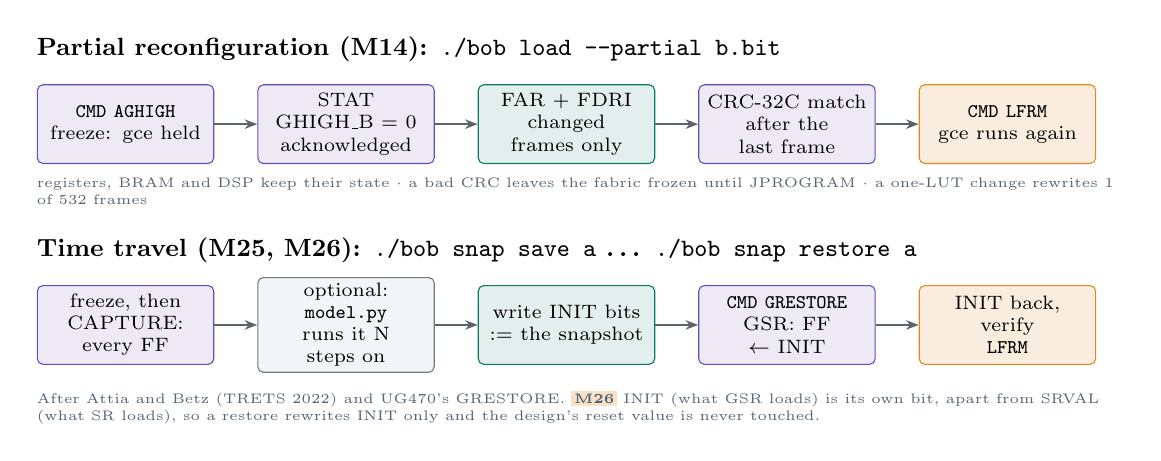
\begin{tikzpicture}[font=\scriptsize, st/.style={bx, minimum height=10mm, text width=21mm}]
    \node[font=\small\bfseries, anchor=west] at (0,5.25) {Partial reconfiguration (M14): \texttt{./bob load -{}-partial b.bit}};
    \node[cfg, st] (p1) at (1.25,4.3) {\texttt{CMD AGHIGH}\\freeze: gce held};
    \node[cfg, st] (p2) at (4.05,4.3) {STAT GHIGH\_B = 0\\acknowledged};
    \node[acc, st] (p3) at (6.85,4.3) {FAR + FDRI\\changed frames only};
    \node[cfg, st] (p4) at (9.65,4.3) {CRC-32C match\\after the last frame};
    \node[hot, st] (p5) at (12.45,4.3) {\texttt{CMD LFRM}\\gce runs again};
    \foreach \a/\b in {p1/p2,p2/p3,p3/p4,p4/p5} \draw[arr] (\a) -- (\b);
    \node[lbl, anchor=west, text width=138mm] at (0,3.45) {registers, BRAM and DSP keep their state $\cdot$ a bad CRC leaves the fabric frozen until JPROGRAM $\cdot$ a one-LUT change rewrites 1 of 532 frames};
    \node[font=\small\bfseries, anchor=west] at (0,2.7) {Time travel (M25, M26): \texttt{./bob snap save a} \dots\ \texttt{./bob snap restore a}};
    \node[cfg, st] (t1) at (1.25,1.75) {freeze, then\\CAPTURE: every FF};
    \node[blk, st] (t2) at (4.05,1.75) {optional: \texttt{model.py}\\runs it N steps on};
    \node[acc, st] (t3) at (6.85,1.75) {write INIT bits\\:= the snapshot};
    \node[cfg, st] (t4) at (9.65,1.75) {\texttt{CMD GRESTORE}\\GSR: FF $\leftarrow$ INIT};
    \node[hot, st] (t5) at (12.45,1.75) {INIT back, verify\\\texttt{LFRM}};
    \foreach \a/\b in {t1/t2,t2/t3,t3/t4,t4/t5} \draw[arr] (\a) -- (\b);
    \node[lbl, anchor=west, text width=138mm] at (0,0.7) {After Attia and Betz (TRETS 2022) and UG470's GRESTORE. \mtag{M26} INIT (what GSR loads) is its own bit, apart from SRVAL (what SR loads), so a restore rewrites INIT only and the design's reset value is never touched.};
  \end{tikzpicture}
\end{frame}

% =============================================================================
\begin{frame}{Observability: every register, every pin, every frame}
  \centering
  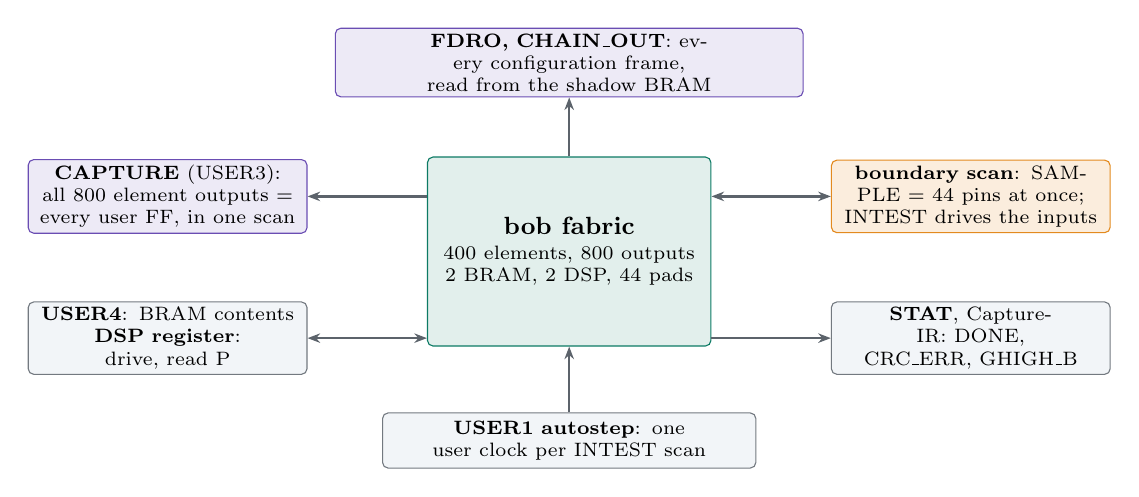
\begin{tikzpicture}[font=\scriptsize]
    \node[acc, minimum width=36mm, minimum height=24mm] (fab) at (7,2.6) {\small\textbf{bob fabric}\\[1pt]400 elements, 800 outputs\\2 BRAM, 2 DSP, 44 pads};
    \node[cfg, text width=58mm] (rb) at (7,5.0) {\textbf{FDRO, CHAIN\_OUT}: every configuration frame,\\read from the shadow BRAM};
    \node[cfg, text width=34mm] (cap) at (1.9,3.3) {\textbf{CAPTURE} (USER3): all 800 element outputs = every user FF, in one scan};
    \node[hot, text width=34mm] (bs) at (12.1,3.3) {\textbf{boundary scan}: SAMPLE = 44 pins at once; INTEST drives the inputs};
    \node[blk, text width=34mm] (u4) at (1.9,1.5) {\textbf{USER4}: BRAM contents\\\textbf{DSP register}: drive, read P};
    \node[blk, text width=34mm] (stt) at (12.1,1.5) {\textbf{STAT}, Capture-IR: DONE, CRC\_ERR, GHIGH\_B};
    \node[blk, text width=46mm] (as) at (7,0.2) {\textbf{USER1 autostep}: one user clock per INTEST scan};
    \draw[arr] (fab.north) -- (rb.south);
    \draw[arr] (fab.west |- cap.east) -- (cap.east);
    \draw[arr2] (fab.east |- bs.west) -- (bs.west);
    \draw[arr2] (fab.west |- u4.east) -- (u4.east);
    \draw[arr] (fab.east |- stt.west) -- (stt.west);
    \draw[arr] (as.north) -- (fab.south);
  \end{tikzpicture}
  \vspace{2mm}

  \small Used by: \texttt{hwtest.py} (board $=$ model after every clock) $\cdot$ \texttt{padwave.py} (a logic analyser on the pads, VCD) $\cdot$ \texttt{snapshot.py} (time travel) $\cdot$ bob studio's Debug view
\end{frame}

% =============================================================================
\section{Software}
\begin{frame}{Software structure: five layers}
  \centering
  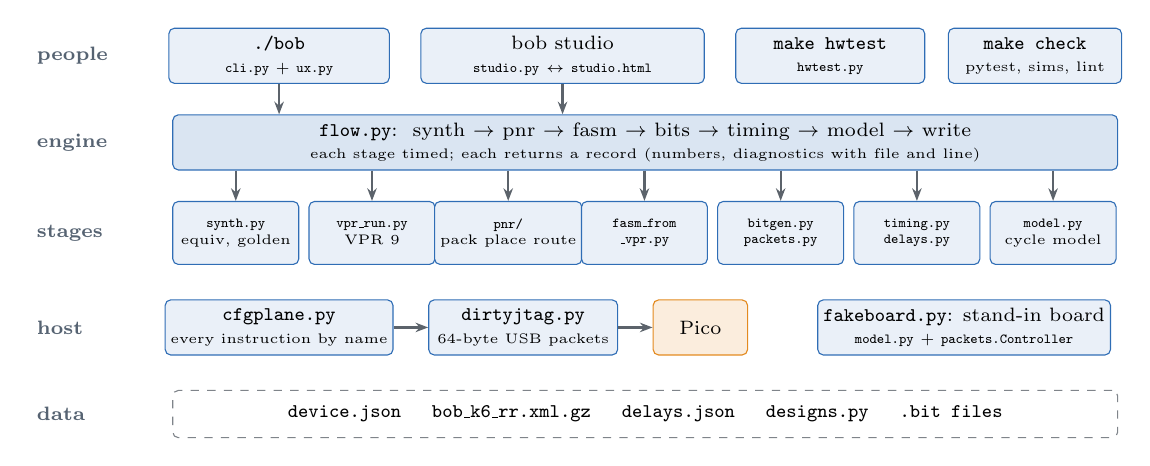
\begin{tikzpicture}[font=\scriptsize]
    \foreach \y/\tx in {5.0/people, 3.9/engine, 2.75/stages, 1.55/host, 0.45/data}
      \node[anchor=west, font=\scriptsize\bfseries, text=bobmute] at (0,\y) {\tx};
    \node[sw, minimum width=28mm] (cli) at (3.2,5.0) {\texttt{./bob}\\\tiny \texttt{cli.py} + \texttt{ux.py}};
    \node[sw, minimum width=36mm] (stu) at (6.8,5.0) {bob studio\\\tiny \texttt{studio.py} $\leftrightarrow$ \texttt{studio.html}};
    \node[sw, minimum width=24mm] (hwt) at (10.2,5.0) {\texttt{make hwtest}\\\tiny \texttt{hwtest.py}};
    \node[sw, minimum width=22mm] (chk) at (12.8,5.0) {\texttt{make check}\\\tiny pytest, sims, lint};
    \node[sw, minimum width=120mm, fill=bobblue!18] (flow) at (7.85,3.9) {\texttt{flow.py}:\ \ synth $\rightarrow$ pnr $\rightarrow$ fasm $\rightarrow$ bits $\rightarrow$ timing $\rightarrow$ model $\rightarrow$ write\\\tiny each stage timed; each returns a record (numbers, diagnostics with file and line)};
    \foreach \nm/\x/\tx in {s1/2.65/{\texttt{synth.py}\\equiv, golden}, s2/4.38/{\texttt{vpr\_run.py}\\VPR 9}, s3/6.11/{\texttt{pnr/}\\pack place route}, s4/7.84/{\texttt{fasm\_from}\\\texttt{\_vpr.py}}, s5/9.57/{\texttt{bitgen.py}\\\texttt{packets.py}}, s6/11.3/{\texttt{timing.py}\\\texttt{delays.py}}, s7/13.03/{\texttt{model.py}\\cycle model}}
    {
      \node[sw, font=\tiny, minimum width=16mm, minimum height=8mm] (\nm) at (\x,2.75) {\tx};
      \draw[arr] (flow.south -| \nm.north) -- (\nm.north);
    }
    \node[sw, minimum width=26mm] (cp) at (3.2,1.55) {\texttt{cfgplane.py}\\\tiny every instruction by name};
    \node[sw, minimum width=24mm] (dj) at (6.3,1.55) {\texttt{dirtyjtag.py}\\\tiny 64-byte USB packets};
    \node[hot, minimum width=12mm] (pico) at (8.55,1.55) {Pico};
    \node[sw, minimum width=34mm] (fk) at (11.9,1.55) {\texttt{fakeboard.py}: stand-in board\\\tiny \texttt{model.py} + \texttt{packets.Controller}};
    \draw[arr] (cp) -- (dj); \draw[arr] (dj) -- (pico);
    \node[file, minimum width=120mm, font=\scriptsize\ttfamily] (data) at (7.85,0.45) {device.json \quad bob\_k6\_rr.xml.gz \quad delays.json \quad designs.py \quad .bit files};
    \draw[arr] (cli.south) -- (cli.south |- flow.north);
    \draw[arr] (stu.south) -- (stu.south |- flow.north);
  \end{tikzpicture}
  \vspace{1mm}

  \small Every user surface drives the same \texttt{flow.py} and \texttt{cfgplane.py}: \texttt{tests/test\_flow.py} requires \texttt{flow.py} and \texttt{./bob build} to write a \textbf{byte-identical} \texttt{.bit}.
\end{frame}

% =============================================================================
\begin{frame}{The guest flow: what each stage takes and hands on}
  \centering
  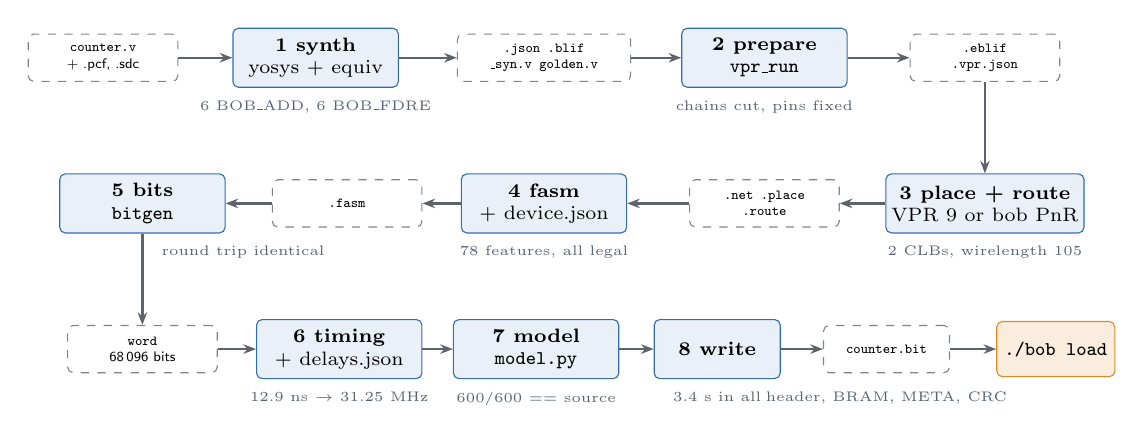
\begin{tikzpicture}[font=\scriptsize, proc/.style={sw, minimum width=21mm, minimum height=7.5mm}, dat/.style={file, minimum width=19mm}, res/.style={lbl, anchor=north}]
    % row 1
    \node[dat] (v) at (1.1,4.7) {counter.v\\\sffamily + .pcf, .sdc};
    \node[proc] (s1) at (3.8,4.7) {\textbf{1 synth}\\yosys + equiv};
    \node[dat, minimum width=22mm] (nl) at (6.7,4.7) {.json .blif\\\_syn.v golden.v};
    \node[proc] (s2) at (9.5,4.7) {\textbf{2 prepare}\\\texttt{vpr\_run}};
    \node[dat] (eb) at (12.3,4.7) {.eblif\\.vpr.json};
    % row 2 (right to left)
    \node[proc, minimum width=24mm] (s3) at (12.3,2.85) {\textbf{3 place + route}\\VPR 9 or bob PnR};
    \node[dat] (pr) at (9.5,2.85) {.net .place\\.route};
    \node[proc] (s4) at (6.7,2.85) {\textbf{4 fasm}\\+ device.json};
    \node[dat] (fa) at (4.2,2.85) {.fasm};
    \node[proc] (s5) at (1.6,2.85) {\textbf{5 bits}\\\texttt{bitgen}};
    % row 3
    \node[dat] (w) at (1.6,1.0) {word\\\sffamily 68\,096 bits};
    \node[proc] (s6) at (4.1,1.0) {\textbf{6 timing}\\+ delays.json};
    \node[proc] (s7) at (6.6,1.0) {\textbf{7 model}\\\texttt{model.py}};
    \node[proc, minimum width=16mm] (s8) at (8.9,1.0) {\textbf{8 write}};
    \node[dat, minimum width=16mm] (bit) at (11.05,1.0) {counter.bit};
    \node[hot, minimum width=15mm] (ld) at (13.2,1.0) {\texttt{./bob load}};
    \foreach \a/\b in {v/s1,s1/nl,nl/s2,s2/eb,eb/s3,s3/pr,pr/s4,s4/fa,fa/s5,s5/w,w/s6,s6/s7,s7/s8,s8/bit,bit/ld} \draw[arr] (\a) -- (\b);
    % results for the counter
    \node[res] at (3.8,4.28) {6 BOB\_ADD, 6 BOB\_FDRE};
    \node[res] at (9.5,4.28) {chains cut, pins fixed};
    \node[res] at (12.3,2.43) {2 CLBs, wirelength 105};
    \node[res] at (6.7,2.43) {78 features, all legal};
    \node[res, anchor=north west] at (1.72,2.43) {round trip identical};
    \node[res] at (4.1,0.58) {12.9 ns $\rightarrow$ 31.25 MHz};
    \node[res] at (6.6,0.58) {600/600 == source};
    \node[res] at (8.9,0.58) {3.4 s in all};
    \node[res] at (11.05,0.58) {header, BRAM, META, CRC};
  \end{tikzpicture}
  \vspace{2mm}

  \small Solid: a stage of \texttt{flow.py}, each one checked before the next runs. Dashed: what it hands on. Grey: the counter at M26.
\end{frame}

% =============================================================================
\begin{frame}{Stage 1, synthesis: yosys onto bob's cells (\texttt{synth.py})}
  \begin{columns}[T]
    \column{0.52\textwidth}
    \centering
    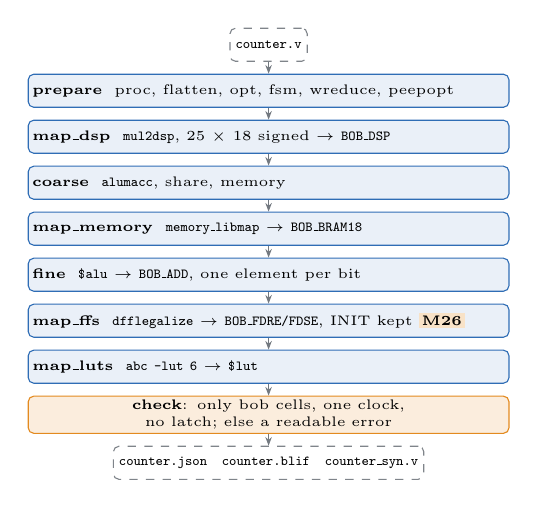
\begin{tikzpicture}[font=\tiny, node distance=1.5mm, ypass/.style={sw, minimum height=4.2mm, text width=60mm, align=left, font=\tiny, inner sep=1.5pt}, dn/.style={-{Stealth[length=1.1mm]}, color=bobink!60}]
      \node[file, minimum height=4.2mm] (src) {counter.v};
      \node[ypass,below=of src] (s1) {\textbf{prepare}\ \ proc, flatten, opt, fsm, wreduce, peepopt};
      \node[ypass,below=of s1] (s2) {\textbf{map\_dsp}\ \ \texttt{mul2dsp}, 25 $\times$ 18 signed $\rightarrow$ \texttt{BOB\_DSP}};
      \node[ypass,below=of s2] (s3) {\textbf{coarse}\ \ \texttt{alumacc}, share, memory};
      \node[ypass,below=of s3] (s4) {\textbf{map\_memory}\ \ \texttt{memory\_libmap} $\rightarrow$ \texttt{BOB\_BRAM18}};
      \node[ypass,below=of s4] (s5) {\textbf{fine}\ \ \texttt{\$alu} $\rightarrow$ \texttt{BOB\_ADD}, one element per bit};
      \node[ypass,below=of s5] (s6) {\textbf{map\_ffs}\ \ \texttt{dfflegalize} $\rightarrow$ \texttt{BOB\_FDRE/FDSE}, INIT kept \mtag{M26}};
      \node[ypass,below=of s6] (s7) {\textbf{map\_luts}\ \ \texttt{abc -lut 6} $\rightarrow$ \texttt{\$lut}};
      \node[hot, below=of s7, text width=60mm, minimum height=4.2mm, font=\tiny, inner sep=1.5pt] (ck) {\textbf{check}: only bob cells, one clock, no latch; else a readable error};
      \node[file, below=of ck, minimum height=4.2mm] (out) {counter.json\quad counter.blif\quad counter\_syn.v};
      \foreach \a/\b in {src/s1,s1/s2,s2/s3,s3/s4,s4/s5,s5/s6,s6/s7,s7/ck,ck/out} \draw[dn] (\a) -- (\b);
    \end{tikzpicture}
    \column{0.46\textwidth}
    \scriptsize
    \begin{tabular}{@{}ll@{}}
      \toprule
      bob cell & becomes \\
      \midrule
      \texttt{\$lut} (K $\leq$ 6) & element LUT, O6 or O5 \\
      \texttt{BOB\_ADD} & element carry, or Double Duty \\
      \texttt{BOB\_FDRE/FDSE} & element FF (INIT, SRVAL) \\
      \texttt{BOB\_BRAM18} & BRAM tile \\
      \texttt{BOB\_DSP} & DSP tile \\
      \bottomrule
    \end{tabular}
    \vspace{3mm}

    \footnotesize
    \begin{itemize}
      \item \textbf{counter}: 6 \texttt{BOB\_ADD} + 6 \texttt{BOB\_FDRE}, 0 LUTs
      \item Then \texttt{equiv.py}: source $\parallel$ netlist $\parallel$ golden netlist in iverilog, 300 biased random cycles
      \item \texttt{golden.py}: one named wire per bit, so CAPTURE bit $i$ = golden register $n$
      \item Why: \texttt{synth\_xilinx}'s proven pass order with bob's cells swapped in
    \end{itemize}
  \end{columns}
\end{frame}

% =============================================================================
\begin{frame}{Stages 2--3: prepare, then two place-and-route engines}
  \centering
  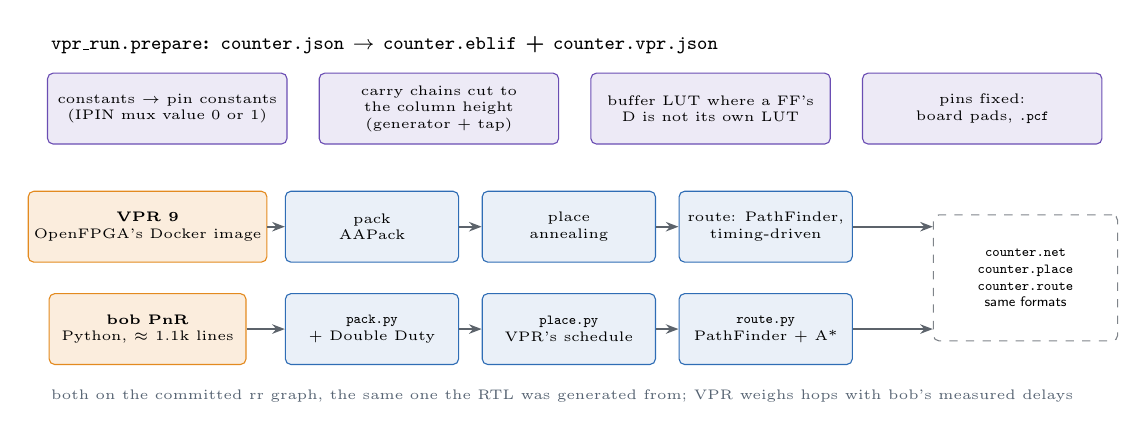
\begin{tikzpicture}[font=\scriptsize, prep/.style={cfg, text width=29mm, font=\tiny, minimum height=9mm}, eng/.style={sw, minimum width=22mm, minimum height=9mm, font=\tiny}]
    \node[font=\scriptsize\bfseries, anchor=west] at (0,5.55) {\texttt{vpr\_run.prepare}: \texttt{counter.json} $\rightarrow$ \texttt{counter.eblif} + \texttt{counter.vpr.json}};
    \node[prep] (q1) at (1.6,4.75) {constants $\rightarrow$ pin constants (IPIN mux value 0 or 1)};
    \node[prep] (q2) at (5.05,4.75) {carry chains cut to the column height (generator + tap)};
    \node[prep] (q3) at (8.5,4.75) {buffer LUT where a FF's D is not its own LUT};
    \node[prep] (q4) at (11.95,4.75) {pins fixed: board pads, \texttt{.pcf}};
    \node[hot, minimum width=25mm, minimum height=9mm, font=\tiny] (vl) at (1.35,3.25) {\textbf{VPR 9}\\OpenFPGA's Docker image};
    \node[eng] (v1) at (4.2,3.25) {pack\\AAPack};
    \node[eng] (v2) at (6.7,3.25) {place\\annealing};
    \node[eng] (v3) at (9.2,3.25) {route: PathFinder,\\timing-driven};
    \node[hot, minimum width=25mm, minimum height=9mm, font=\tiny] (bl) at (1.35,1.95) {\textbf{bob PnR}\\Python, $\approx$ 1.1k lines};
    \node[eng] (b1) at (4.2,1.95) {\texttt{pack.py}\\+ Double Duty};
    \node[eng] (b2) at (6.7,1.95) {\texttt{place.py}\\VPR's schedule};
    \node[eng] (b3) at (9.2,1.95) {\texttt{route.py}\\PathFinder + A*};
    \node[file, minimum height=16mm, text width=22mm] (o) at (12.5,2.6) {counter.net\\counter.place\\counter.route\\\sffamily same formats};
    \foreach \a/\b in {vl/v1,v1/v2,v2/v3,bl/b1,b1/b2,b2/b3} \draw[arr] (\a) -- (\b);
    \draw[arr] (v3.east) -- (o.west |- v3.east);
    \draw[arr] (b3.east) -- (o.west |- b3.east);
    \node[lbl, anchor=west] at (0,1.1) {both on the committed rr graph, the same one the RTL was generated from; VPR weighs hops with bob's measured delays};
  \end{tikzpicture}
  \vspace{2mm}

  \kpi{0.87$\times$}{bob's wirelength vs VPR\\13 designs}\hfill
  \kpi{$-$13.2\,\%}{elements with Double Duty\\(VPR's packer: $-$4.7\,\%)}\hfill
  \kpi{11 iterations}{\texttt{fir16}: 40 CLBs\\routed in 6.1 s}\hfill
  \kpi{both}{flows pass on the board\\(\texttt{pnr-*} checks)}
\end{frame}

% =============================================================================
\begin{frame}[fragile]{Stages 4--5, FASM and bitgen: from a route to a frame}
  \begin{columns}[T]
    \column{0.44\textwidth}
    \textbf{\scriptsize counter.fasm (78 features; excerpt)}
{\tiny
\begin{verbatim}
clb_x7y2.e0.cy_en    = 1'h1
clb_x7y2.e0.dd       = 1'h1
clb_x7y2.e1.ff_en    = 1'h1
clb_x7y2.e1.ff_ce_en = 1'h1
clb_x7y2.e1.x5       = 5'h14
rr1924               = 3'h2
rr6840               = 2'h2
\end{verbatim}
}
    \textbf{\scriptsize gates.fasm (a fractured LUT)}
{\tiny
\begin{verbatim}
clb_x1y3.e2.frac = 1'h1
clb_x1y3.e2.init = 64'hcccc0000ffee5544
\end{verbatim}
}
    \scriptsize
    A feature is \texttt{block.field = value}; names come from \texttt{device.py}'s fields; every line is checked against \texttt{device.json}.
    \column{0.54\textwidth}
    \centering
    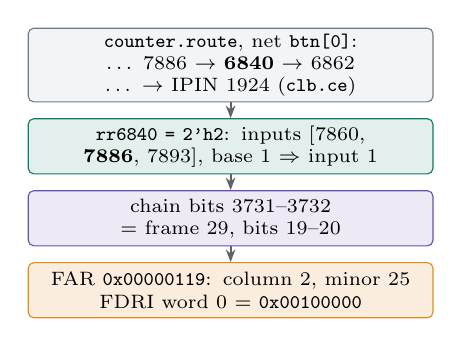
\begin{tikzpicture}[font=\tiny, node distance=2mm]
      \node[blk, text width=50mm] (r) {\texttt{counter.route}, net \texttt{btn[0]}:\\\dots\ 7886 $\rightarrow$ \textbf{6840} $\rightarrow$ 6862 \dots\ $\rightarrow$ IPIN 1924 (\texttt{clb.ce})};
      \node[acc, below=of r, text width=50mm] (f) {\texttt{rr6840 = 2'h2}: inputs [7860, \textbf{7886}, 7893], base 1 $\Rightarrow$ input 1};
      \node[cfg, below=of f, text width=50mm] (b) {chain bits 3731--3732 = frame 29, bits 19--20};
      \node[hot, below=of b, text width=50mm] (a) {FAR \texttt{0x00000119}: column 2, minor 25\\FDRI word 0 = \texttt{0x00100000}};
      \draw[arr] (r)--(f); \draw[arr] (f)--(b); \draw[arr] (b)--(a);
    \end{tikzpicture}
    \vspace{2mm}

    \raggedright\scriptsize
    \begin{itemize}
      \item \texttt{bitgen.py}: FASM $\leftrightarrow$ 68\,096-bit word, an exact round trip
      \item \texttt{.bit} = header, configuration, a BRAM section per used memory, META (sources, hashes, clock), file CRC
      \item \texttt{packets.py} turns the word into the stream of the packet slide
    \end{itemize}
  \end{columns}
\end{frame}

% =============================================================================
\begin{frame}{Stage 6, timing: signed off from the configured bits}
  \begin{columns}[T]
    \column{0.5\textwidth}
    \footnotesize
    \textbf{Why Vivado cannot do it}
    \begin{itemize}
      \item An \emph{unconfigured} fabric is a mesh of combinational loops (M21: a 6\,349-level path through empty muxes)
      \item So the XDC relaxes the fabric paths, and \texttt{timing.py} times each design from its own bits
    \end{itemize}
    \textbf{How} (\texttt{timing.py}, after ZUMA and ARC 2021)
    \begin{itemize}
      \item Walk only the \emph{selected} mux inputs, register to register; one delay per hop class
      \item The \textbf{contract}: a build or load is refused unless path $\times$ guard fits the design's gce spacing; a loop is refused too
    \end{itemize}
    \column{0.48\textwidth}
    \footnotesize
    \textbf{Delays measured in Vivado} (\texttt{delays.tcl})
    \vspace{1mm}

    \centering
    \scriptsize
    \begin{tabular}{@{}lrl@{}}
      \toprule
      hop & delay & source \\
      \midrule
      routing mux & 4.60 ns & max of 32 samples \\
      input mux & 4.65 ns & max of 53 samples \\
      crossbar mux & 3.01 ns & max of 91 samples \\
      element (LUT) & 3.4 ns & estimate \\
      carry, per element & 1.0 ns & estimate \\
      FF clk$\rightarrow$Q / setup & 0.5 / 1.0 ns & estimate \\
      \bottomrule
    \end{tabular}

    \raggedright
    \src{Estimates keep a 2$\times$ guard band (1.25$\times$ once all are measured). VPR places and routes on these same numbers.}

    \vspace{3mm}
    \textbf{\footnotesize The counter's critical path}\\[1mm]
    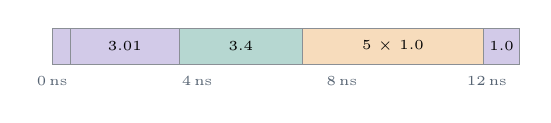
\begin{tikzpicture}[x=4.6mm, y=4.6mm, font=\tiny]
      \foreach \a/\b/\tx/\col in {0/0.5/{}/bobviolet, 0.5/3.509/3.01/bobviolet, 3.509/6.909/3.4/bobteal, 6.909/11.909/5 $\times$ 1.0/bobamber, 11.909/12.909/1.0/bobviolet}
        { \fill[\col!30] (\a,0) rectangle (\b,1); \draw[bobink!50] (\a,0) rectangle (\b,1); \node at ({(\a+\b)/2},0.5) {\tx}; }
      \foreach \xx in {0,4,8,12} \node[color=bobmute] at (\xx,-0.45) {\xx\,ns};
    \end{tikzpicture}\\[1mm]
    {\scriptsize clk$\rightarrow$Q, crossbar, element, carry, setup = 12.909 ns;\\
     $\times$ 2 = 25.8 ns $\rightarrow$ 4 cycles of 8 ns: \textbf{31.25 MHz}}
  \end{columns}
\end{frame}

% =============================================================================
\begin{frame}{Loading: \texttt{./bob load counter.bit}}
  \begin{columns}[T]
    \column{0.55\textwidth}
    \centering
    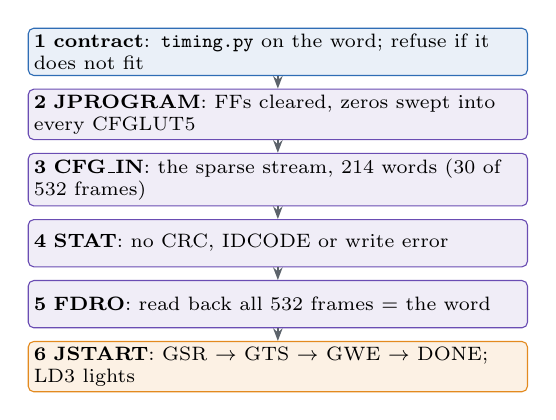
\begin{tikzpicture}[font=\scriptsize, node distance=1.6mm, ldstep/.style={bx, text width=62mm, align=left, minimum height=6mm}]
      \node[ldstep,draw=bobblue, fill=bobblue!10] (a1) {\textbf{1 contract}: \texttt{timing.py} on the word; refuse if it does not fit};
      \node[ldstep,draw=bobviolet, fill=bobviolet!10, below=of a1] (a2) {\textbf{2 JPROGRAM}: FFs cleared, zeros swept into every CFGLUT5};
      \node[ldstep,draw=bobviolet, fill=bobviolet!10, below=of a2] (a3) {\textbf{3 CFG\_IN}: the sparse stream, 214 words (30 of 532 frames)};
      \node[ldstep,draw=bobviolet, fill=bobviolet!10, below=of a3] (a4) {\textbf{4 STAT}: no CRC, IDCODE or write error};
      \node[ldstep,draw=bobviolet, fill=bobviolet!10, below=of a4] (a5) {\textbf{5 FDRO}: read back all 532 frames $=$ the word};
      \node[ldstep,draw=bobamber, fill=bobamber!12, below=of a5] (a6) {\textbf{6 JSTART}: GSR $\rightarrow$ GTS $\rightarrow$ GWE $\rightarrow$ DONE; LD3 lights};
      \foreach \a/\b in {a1/a2,a2/a3,a3/a4,a4/a5,a5/a6} \draw[arr] (\a) -- (\b);
    \end{tikzpicture}

    \vspace{1mm}
    \raggedright
    \src{\texttt{-{}-mode chain}: the same word over CHAIN\_IN with its CRC in CFG\_CTRL. \texttt{-{}-partial}: only the frames that differ.}
    \column{0.43\textwidth}
    \centering
    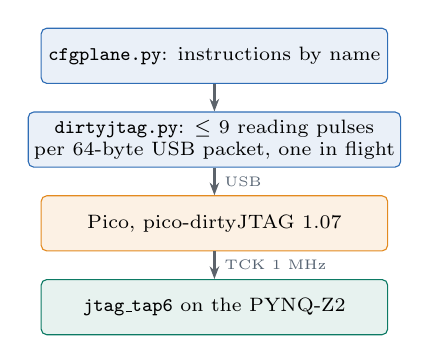
\begin{tikzpicture}[font=\scriptsize, node distance=3.5mm, tier/.style={bx, minimum width=44mm}]
      \node[tier,draw=bobblue, fill=bobblue!10] (c1) {\texttt{cfgplane.py}: instructions by name};
      \node[tier,draw=bobblue, fill=bobblue!10, below=of c1] (c2) {\texttt{dirtyjtag.py}: $\leq$ 9 reading pulses\\per 64-byte USB packet, one in flight};
      \node[tier,draw=bobamber, fill=bobamber!12, below=of c2] (c3) {Pico, pico-dirtyJTAG 1.07};
      \node[tier,draw=bobteal, fill=bobteal!10, below=of c3] (c4) {\texttt{jtag\_tap6} on the PYNQ-Z2};
      \draw[arr] (c1) -- (c2); \draw[arr] (c2) -- node[right, lbl]{USB} (c3); \draw[arr] (c3) -- node[right, lbl]{TCK 1 MHz} (c4);
    \end{tikzpicture}
    \vspace{2mm}

    \kpi{2.9$\times$}{13 designs: 28.2 s at 100 kHz,\\9.8 s at 1 MHz}

    \vspace{1mm}
    \raggedright
    \src{\texttt{-{}-probe fake}: \texttt{fakeboard.py} answers the same JTAG out of \texttt{model.py} and \texttt{packets.Controller}.}
  \end{columns}
\end{frame}

% =============================================================================
\begin{frame}{bob studio: an EDA tool over the same engine}
  \centering
  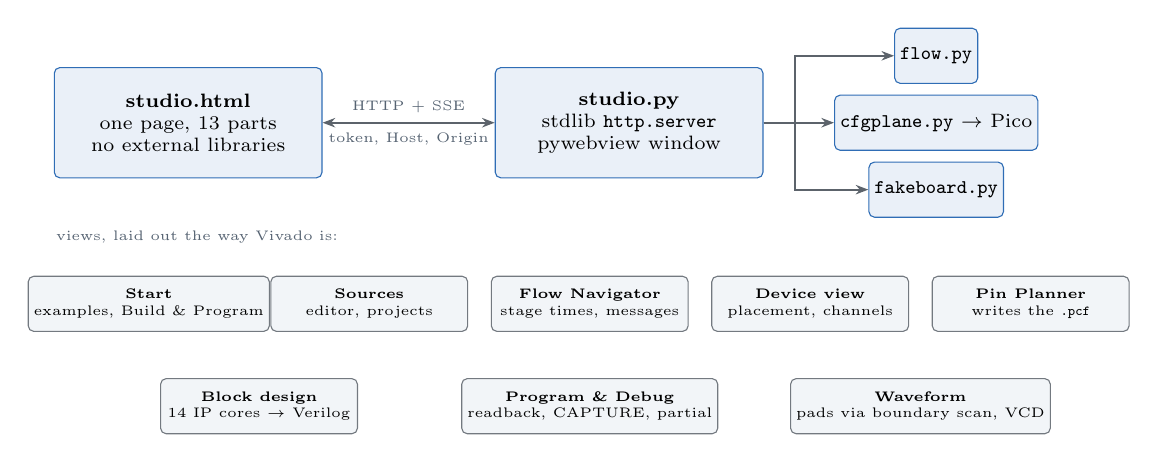
\begin{tikzpicture}[font=\scriptsize]
    \node[sw, minimum width=34mm, minimum height=14mm] (pg) at (1.8,3.9) {\textbf{studio.html}\\one page, 13 parts\\no external libraries};
    \node[sw, minimum width=34mm, minimum height=14mm] (be) at (7.4,3.9) {\textbf{studio.py}\\stdlib \texttt{http.server}\\pywebview window};
    \draw[arr2] (pg) -- node[above, lbl]{HTTP + SSE} node[below, lbl]{token, Host, Origin} (be);
    \node[sw] (fl) at (11.3,4.75) {\texttt{flow.py}};
    \node[sw] (cp) at (11.3,3.9) {\texttt{cfgplane.py} $\rightarrow$ Pico};
    \node[sw] (fk) at (11.3,3.05) {\texttt{fakeboard.py}};
    \draw[arr] (be.east) -- ++(0.4,0) |- (fl.west);
    \draw[arr] (be.east) -- (cp.west);
    \draw[arr] (be.east) -- ++(0.4,0) |- (fk.west);
    \foreach \nm/\x/\y/\tx in {
      v1/1.3/1.6/{\textbf{Start}\\examples, Build \& Program},
      v2/4.1/1.6/{\textbf{Sources}\\editor, projects},
      v3/6.9/1.6/{\textbf{Flow Navigator}\\stage times, messages},
      v4/9.7/1.6/{\textbf{Device view}\\placement, channels},
      v5/12.5/1.6/{\textbf{Pin Planner}\\writes the \texttt{.pcf}},
      v6/2.7/0.3/{\textbf{Block design}\\14 IP cores $\rightarrow$ Verilog},
      v7/6.9/0.3/{\textbf{Program \& Debug}\\readback, CAPTURE, partial},
      v8/11.1/0.3/{\textbf{Waveform}\\pads via boundary scan, VCD}}
    { \node[blk, minimum width=25mm, font=\tiny] (\nm) at (\x,\y) {\tx}; }
    \node[lbl, anchor=west] at (0,2.45) {views, laid out the way Vivado is:};
  \end{tikzpicture}
  \vspace{2mm}

  \small \texttt{./bob studio} (\texttt{-{}-probe fake} without a board). It never re-implements a stage: every route calls \texttt{flow.py} or \texttt{cfgplane.py}.
\end{frame}

% =============================================================================
\section{Why, and OpenFPGA}
\begin{frame}{Verification: expected values never come from the RTL}
  \centering
  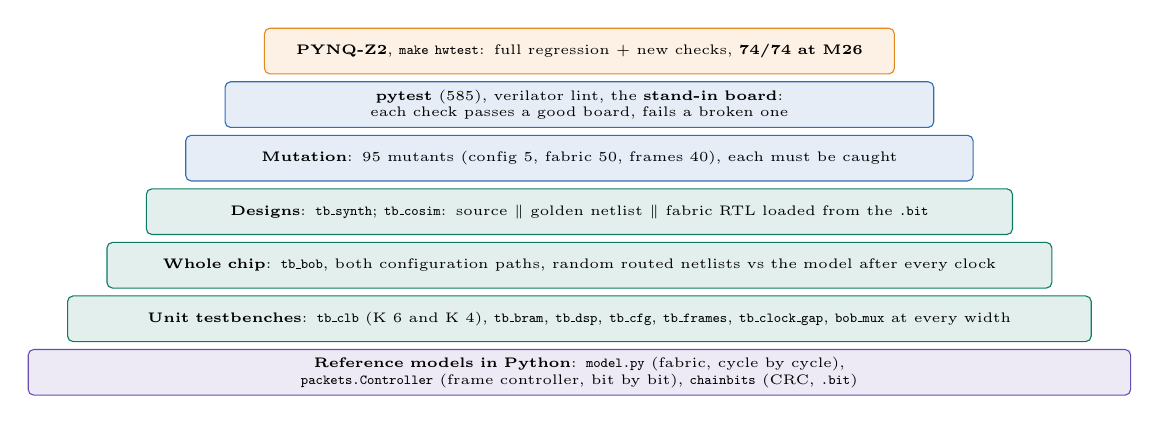
\begin{tikzpicture}[font=\tiny]
    \foreach \i/\w/\tw/\col/\tx in {
      0/14cm/13.6cm/bobviolet/{\textbf{Reference models in Python}: \texttt{model.py} (fabric, cycle by cycle), \texttt{packets.Controller} (frame controller, bit by bit), \texttt{chainbits} (CRC, \texttt{.bit})},
      1/13cm/12.6cm/bobteal/{\textbf{Unit testbenches}: \texttt{tb\_clb} (K 6 and K 4), \texttt{tb\_bram}, \texttt{tb\_dsp}, \texttt{tb\_cfg}, \texttt{tb\_frames}, \texttt{tb\_clock\_gap}, \texttt{bob\_mux} at every width},
      2/12cm/11.6cm/bobteal/{\textbf{Whole chip}: \texttt{tb\_bob}, both configuration paths, random routed netlists vs the model after every clock},
      3/11cm/10.6cm/bobteal/{\textbf{Designs}: \texttt{tb\_synth}; \texttt{tb\_cosim}: source $\parallel$ golden netlist $\parallel$ fabric RTL loaded from the \texttt{.bit}},
      4/10cm/9.6cm/bobblue/{\textbf{Mutation}: 95 mutants (config 5, fabric 50, frames 40), each must be caught},
      5/9cm/8.6cm/bobblue/{\textbf{pytest} (585), verilator lint, the \textbf{stand-in board}: each check passes a good board, fails a broken one},
      6/8cm/7.6cm/bobamber/{\textbf{PYNQ-Z2}, \texttt{make hwtest}: full regression + new checks, \textbf{74/74 at M26}}}
    {
      \node[draw=\col, fill=\col!12, rounded corners=2pt, minimum width=\w, text width=\tw, align=center, minimum height=5.8mm, inner sep=1.2pt] at (0,\i*0.68) {\tx};
    }
  \end{tikzpicture}
  \vspace{2mm}

  \small A testbench that reads its answers off the RTL only proves the RTL agrees with itself.\\
  Mutants prove the \emph{guards} are tested: M2's first length check could be deleted unnoticed.
\end{frame}

% =============================================================================
\begin{frame}{The tool stack: what, and why}
  \centering
  \scriptsize
  \renewcommand{\arraystretch}{1.2}
  \begin{tabular}{@{}L{30mm}L{40mm}L{60mm}@{}}
    \toprule
    \textbf{what} & \textbf{used for} & \textbf{why} \\
    \midrule
    yosys & synthesis onto bob's cells & open; \texttt{synth\_xilinx}'s pass order; techmap onto our own cells \\
    VPR 9 (OpenFPGA's Docker image) & rr graph, pack, place, route & the reference academic flow; it writes out its own routing graph \\
    Python 3, standard library & device, models, PnR, bitgen, host, studio & small enough to read; no dependencies to install \\
    Icarus Verilog, Verilator & simulation, lint & open and fast; one source list (\texttt{hw/sources.f}) \\
    Vivado 2025.2 & the host bitstream only & the only way into the XC7Z020; never needed for a guest design \\
    Pico + pico-dirtyJTAG & the USB-JTAG probe & cheap, open firmware, bit-level control of TCK/TMS/TDI \\
    FASM & text form of a configuration & F4PGA's format: readable, diffable, checkable \\
    UG470/473/474/479, IEEE 1149.1 & the semantics followed & packets, CRC, FAR, INIT/SRVAL, TAP: real-world behaviour \\
    pywebview & bob studio as a desktop app & a native window over the same local page \\
    \bottomrule
  \end{tabular}
\end{frame}

% =============================================================================
\begin{frame}{Design decisions: what was chosen, and the evidence}
  \centering
  \scriptsize
  \renewcommand{\arraystretch}{1.1}
  \begin{tabular}{@{}L{40mm}L{32mm}L{58mm}@{}}
    \toprule
    \textbf{chosen} & \textbf{instead of} & \textbf{because} \\
    \midrule
    fabric generated from VPR's rr graph & hand-written routing & router and hardware are one object; every route is loadable \\
    user clock = enable on sysclk & derived or gated clocks & one real clock; cycle-exact stepping; freeze for PR and snapshots \\
    tables + crossbar in CFGLUT5 & config FFs + muxes & a CLB 469 $\rightarrow$ 193 host LUTs (ZUMA's idea) \\
    OR roots; LUT6/MUXF7/MUXF8 muxes & CFGLUT5 roots; inferred muxes & 152 $\rightarrow$ 128 CFGLUT5 per CLB; 10 $\times$ 10 fits \\
    one 128-bit frame buffer & part-select over the memory & the part-select was a 12k-LUT shifter; Vivado ran out of memory \\
    readback from a shadow BRAM & a 256:1 $\times$ 128 mux & $-$11.8k LUTs, a third of the design \\
    UG470 packets, chain kept & a single protocol & self-syncing, addressable, CRC + IDCODE; two paths cross-check \\
    N = 4, full crossbar & N = 10 (OpenFPGA's reference) & measured sweep of host cost per guest LUT \\
    timing per configuration & Vivado's STA & Vivado only sees the unconfigured loops \\
    Double Duty elements & adder and LUT exclusive & $-$13.2\,\% elements with bob's packer \\
    \bottomrule
  \end{tabular}
\end{frame}

% =============================================================================
\begin{frame}{bob and OpenFPGA: the same core, different goals}
  \centering
  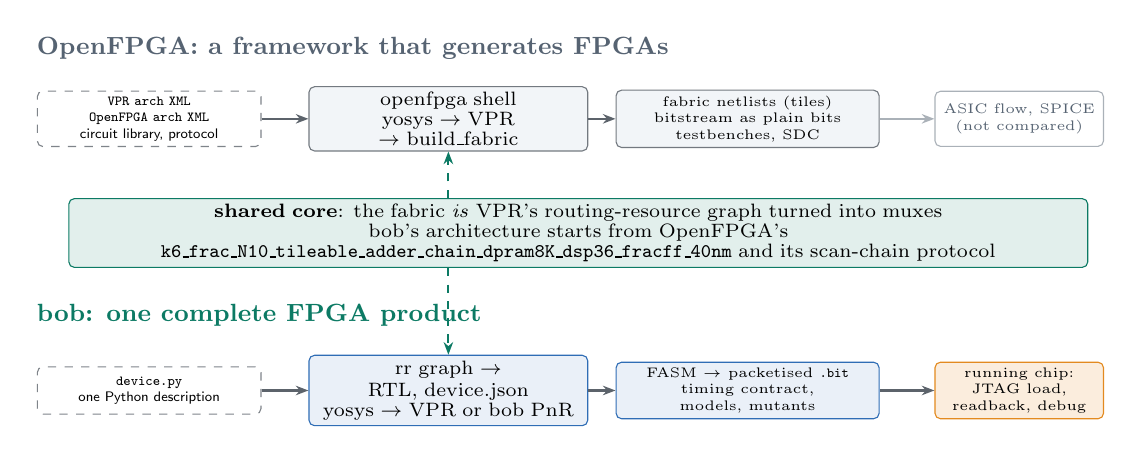
\begin{tikzpicture}[font=\scriptsize]
    \node[font=\small\bfseries, anchor=west, text=bobmute] at (0,5.35) {OpenFPGA: a framework that generates FPGAs};
    \node[file, text width=27mm, font=\tiny\ttfamily] (o1) at (1.55,4.45) {VPR arch XML\\OpenFPGA arch XML\\\sffamily circuit library, protocol};
    \node[blk, text width=34mm, font=\tiny] (o2) at (5.35,4.45) {\scriptsize openfpga shell\\yosys $\rightarrow$ VPR $\rightarrow$ build\_fabric};
    \node[blk, text width=32mm, font=\tiny] (o3) at (9.15,4.45) {fabric netlists (tiles)\\bitstream as plain bits\\testbenches, SDC};
    \node[blk, text width=20mm, font=\tiny, draw=bobmute!50, fill=white, text=bobmute] (o4) at (12.6,4.45) {ASIC flow, SPICE\\(not compared)};
    \draw[arr] (o1) -- (o2); \draw[arr] (o2) -- (o3); \draw[arr, bobmute!50] (o3) -- (o4);
    \node[acc, text width=128mm, minimum height=8mm, font=\tiny] (core) at (7,3.0) {\scriptsize\textbf{shared core}: the fabric \emph{is} VPR's routing-resource graph turned into muxes\\bob's architecture starts from OpenFPGA's \texttt{k6\_frac\_N10\_tileable\_adder\_chain\_dpram8K\_dsp36\_fracff\_40nm} and its scan-chain protocol};
    \node[font=\small\bfseries, anchor=west, text=bobteal] at (0,1.95) {bob: one complete FPGA product};
    \node[file, text width=27mm, font=\tiny\ttfamily] (b1) at (1.55,1.0) {device.py\\\sffamily one Python description};
    \node[sw, text width=34mm, font=\tiny] (b2) at (5.35,1.0) {\scriptsize rr graph $\rightarrow$ RTL, device.json\\yosys $\rightarrow$ VPR or bob PnR};
    \node[sw, text width=32mm, font=\tiny] (b3) at (9.15,1.0) {FASM $\rightarrow$ packetised \texttt{.bit}\\timing contract, models, mutants};
    \node[hot, text width=20mm, font=\tiny] (b4) at (12.6,1.0) {running chip: JTAG load, readback, debug};
    \draw[arr] (b1) -- (b2); \draw[arr] (b2) -- (b3); \draw[arr] (b3) -- (b4);
    \draw[arr, dashed, bobteal] (core.north -| o2.south) -- (o2.south);
    \draw[arr, dashed, bobteal] (core.south -| b2.north) -- (b2.north);
  \end{tikzpicture}
\end{frame}

% =============================================================================
\begin{frame}{Scorecard, physical design aside}
  \centering
  \scriptsize
  \renewcommand{\arraystretch}{1.12}
  \begin{tabular}{@{}L{44mm}ccL{54mm}@{}}
    \toprule
    & \textbf{OpenFPGA} & \textbf{bob} & \textbf{evidence (OpenFPGA vs bob)} \\
    \midrule
    architecture range & \rate{3} & \rate{1} & {\tiny any VPR arch vs one cluster, L4, 1 BRAM, 1 DSP} \\
    fabric from VPR's rr graph & \rate{3} & \rate{3} & {\tiny the same method (bob: \texttt{fabric\_gen.py})} \\
    configuration protocol & \rate{1} & \rate{3} & {\tiny chain, memory bank, decoders vs UG470 packets} \\
    bitstream format & \rate{1} & \rate{3} & {\tiny plain bits vs \texttt{.bit} with CRC, META; sparse, partial} \\
    loader + readback on hardware & \rate{0} & \rate{3} & {\tiny left to the chip's user vs TAP, Pico, FDRO verify} \\
    partial reconfiguration & \rate{0} & \rate{3} & {\tiny not provided vs AGHIGH freeze, CRC-gated LFRM} \\
    hardware debug & \rate{0} & \rate{3} & {\tiny simulation vs CAPTURE, SAMPLE, analyser, GRESTORE} \\
    timing sign-off per design & \rate{2} & \rate{2} & {\tiny SDC for external STA vs measured delays, contract} \\
    second PnR engine & \rate{0} & \rate{2} & {\tiny VPR only vs VPR + bob's PnR (0.87$\times$ wirelength)} \\
    verification depth & \rate{2} & \rate{3} & {\tiny testbenches vs models, co-sim, mutants, board} \\
    scale, maturity, community & \rate{3} & \rate{1} & {\tiny many chips, tape-outs vs 400 LUTs, one board} \\
    \bottomrule
  \end{tabular}
  \vspace{1mm}

  \src{Our assessment of each project's own scope: OpenFPGA's generated fabrics are programmed by whatever loader the chip's integrator builds.}
\end{frame}

% =============================================================================
\begin{frame}{So: is bob better than OpenFPGA?}
  \begin{columns}[T]
    \column{0.48\textwidth}
    \begin{block}{As a generator of many FPGAs: \textbf{no}}
      \small
      \begin{itemize}
        \item OpenFPGA covers far more architectures: cluster shapes, segment mixes, multi-mode blocks, clock networks
        \item It scales to real chips and has a research community behind it
        \item bob has one fabric shape, sized for one board
      \end{itemize}
    \end{block}
    \column{0.48\textwidth}
    \begin{block}{As a complete, working FPGA: \textbf{yes}}
      \small
      \begin{itemize}
        \item bob covers the layer OpenFPGA leaves out: a real protocol, a loader, readback, partial reconfiguration, debug, timing per design
        \item Every one of 27 milestones was closed on hardware, with a full regression
        \item The whole loop fits in one head
      \end{itemize}
    \end{block}
  \end{columns}
  \vspace{4mm}
  \begin{columns}[T]
    \column{0.96\textwidth}
    \small
    \textbf{Next, borrowed back}: mixed segment lengths and a clock network (OpenFPGA's clock rr graph), connection boxes fixed before a bigger design, an SDC view for a standard STA, and tile grouping if bob ever goes to silicon.
  \end{columns}
\end{frame}

% =============================================================================
\begin{frame}{27 milestones in 14 days, each closed on the board}
  \centering
  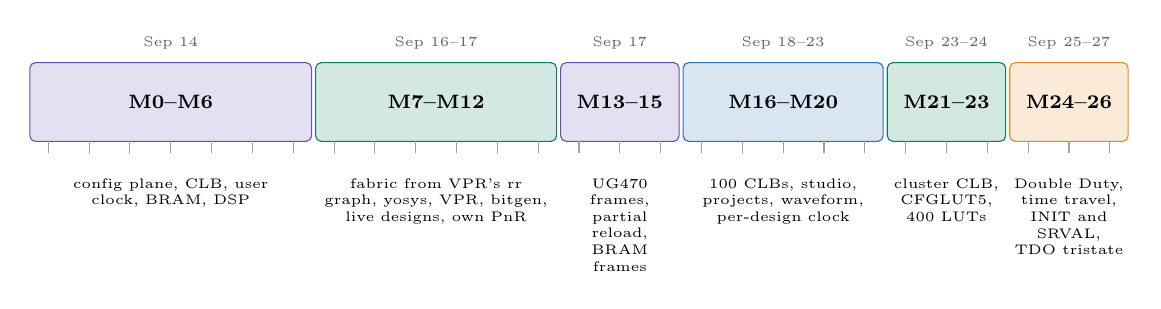
\begin{tikzpicture}[font=\scriptsize, x=5.185mm]
    \foreach \a/\b/\tw/\ti/\dt/\wh/\col in {
      0/7/34mm/{M0--M6}/{Sep 14}/{config plane, CLB, user clock, BRAM, DSP}/bobviolet,
      7/13/29mm/{M7--M12}/{Sep 16--17}/{fabric from VPR's rr graph, yosys, VPR, bitgen, live designs, own PnR}/bobteal,
      13/16/14mm/{M13--15}/{Sep 17}/{UG470 frames, partial reload, BRAM frames}/bobviolet,
      16/21/24mm/{M16--M20}/{Sep 18--23}/{100 CLBs, studio, projects, waveform, per-design clock}/bobblue,
      21/24/14mm/{M21--23}/{Sep 23--24}/{cluster CLB, CFGLUT5, 400 LUTs}/bobteal,
      24/27/14mm/{M24--26}/{Sep 25--27}/{Double Duty, time travel, INIT and SRVAL, TDO tristate}/bobamber}
    {
      \fill[\col!18, draw=\col, rounded corners=2pt] (\a+0.05,2.2) rectangle (\b-0.05,3.2);
      \node[font=\scriptsize\bfseries] at ({(\a+\b)/2},2.7) {\ti};
      \node[lbl] at ({(\a+\b)/2},3.45) {\dt};
      \node[font=\tiny, align=center, anchor=north, text width=\tw] at ({(\a+\b)/2},1.85) {\wh};
    }
    \foreach \m in {0,...,26} \draw[bobmute!60] (\m+0.5,2.2) -- (\m+0.5,2.05);
  \end{tikzpicture}
  \vspace{4mm}

  \small
  \begin{itemize}
    \item Every Vivado build is the complete FPGA plus the new feature; every board run replays all earlier checks first
    \item Board results grew from 11/11 (M0) to \textbf{74/74} (M26); every hardware check was first run against the stand-in board, passing and failing
  \end{itemize}
\end{frame}

% =============================================================================
\begin{frame}{Summary}
  \begin{columns}[T]
    \column{0.32\textwidth}
    \textbf{\color{bobteal}RTL}
    \scriptsize
    \begin{itemize}
      \item 100 CLBs of 4 fracturable LUT6 elements, Double Duty carry, 2 FFs with INIT and SRVAL
      \item Routing generated node for node from VPR's rr graph, on host LUT6/MUXF7/MUXF8
      \item Tables in CFGLUT5; BRAM and DSP on real host blocks
    \end{itemize}
    \column{0.32\textwidth}
    \textbf{\color{bobviolet}Configuration}
    \scriptsize
    \begin{itemize}
      \item 532 frames of 128 bits; UG470-style packets, CRC-32C, IDCODE, STAT
      \item Sparse, partial and chain loads; readback of every frame
      \item Freeze, capture, GRESTORE: time travel
    \end{itemize}
    \column{0.32\textwidth}
    \textbf{\color{bobblue}Software}
    \scriptsize
    \begin{itemize}
      \item One \texttt{device.py} generates arch, RTL and data
      \item yosys $\rightarrow$ VPR or bob PnR $\rightarrow$ FASM $\rightarrow$ bits $\rightarrow$ timing $\rightarrow$ model, every step checked
      \item \texttt{./bob}, bob studio, a Pico loader, a stand-in board
    \end{itemize}
  \end{columns}
  \vspace{6mm}
  \kpi{400}{LUT6}\hfill
  \kpi{8\,095}{configurable muxes}\hfill
  \kpi{68\,096}{configuration bits}\hfill
  \kpi{95}{mutants caught}\hfill
  \kpi{74/74}{board checks, M26}
\end{frame}

% =============================================================================
\begin{frame}[plain]
  \centering
  \vspace{18mm}
  {\Huge\bfseries Thank you}\\[6mm]
  {\large Questions?}\\[12mm]
  \src{Live demo: \texttt{./bob run work/examples/counter/counter.v -{}-probe fake} \quad$\cdot$\quad \texttt{./bob fasm counter.bit} \quad$\cdot$\quad \texttt{./bob studio}}
\end{frame}

\end{document}
